\documentclass[a4paper,12pt]{article}
\usepackage[
    left=30mm,
    right=15mm,
    top=20mm,
    bottom=20mm
]{geometry}
\parindent=1.25cm

%%% Работа с русским языком
\usepackage{cmap}					% поиск в PDF
\usepackage{mathtext} 				% русские буквы в формулах
\usepackage[T2A]{fontenc}           % кодировка
\usepackage[utf8]{inputenc}			% кодировка исходного текста
\usepackage[english,russian]{babel}	% локализация и переносы
\usepackage{indentfirst}
\frenchspacing
\usepackage{setspace}               % межстрочный интервал
\onehalfspacing

%%% Размер шрифта в названиях разделов
\usepackage{sectsty}
\sectionfont{\large}
\subsectionfont{\large}

%%% Дополнительная работа с математикой
\usepackage{amsmath,amsfonts,amssymb,amsthm,mathtools} % AMS
\usepackage{icomma}

%%% Тире в подписях к рисункам
\usepackage{caption}
\captionsetup{labelsep=endash}

%%% Текст в колонки
\usepackage{multicol}

%%% Списки
\usepackage{enumitem}
\setlist{nosep, leftmargin=*}
\renewcommand{\labelenumi}{\arabic*)}

%%% Системы уравнений
\usepackage{cases}

%%% Таблицы
\usepackage{array}

%%% Картинки
\usepackage{graphicx}
\usepackage{float}

%%% Обведение в овал
\usepackage{tikz}
\usetikzlibrary{shapes.misc}
\newcommand*\circled[1]{\tikz[baseline=(char.base)]{\node[shape=rounded rectangle,draw] (char) {#1};}}

%%% Свои имена функций
\DeclareMathOperator{\Div}{div}
\DeclareMathOperator{\Int}{int}
\DeclareMathOperator{\Const}{const}

%%% Список литературы
\bibliographystyle{bibliography_style/gost-numeric.bbx}
\usepackage[
	natbib = true,
	style = gost-numeric,
	sorting = none,
	backend = biber,
	language = autobib,
	autolang = other
]{biblatex}
\addbibresource{../references.bib}

%%% Гиперссылки
\usepackage{hyperref}

%%% Перенос знаков в формулах (по Львовскому)
\newcommand*{\hm}[1]{#1\nobreak\discretionary{}
{\hbox{$\mathsurround=0pt #1$}}{}}

\theoremstyle{plain}
\newtheorem{proposition}{Утверждение}
 
\theoremstyle{definition}
\newtheorem{definition}{Определение}
\newtheorem{remark}{Замечание}
\newtheorem{example}{Пример}


\begin{document}

\begin{abstract}
    Цель настоящей работы -- исследование качественных характеристик и численный анализ модели типа диффузной границы, описывающей развитие канала электрического пробоя в твердом диэлектрике. Проведен анализ устойчивости положений равновесия системы; установлены условия развития канала пробоя из малых возмущений неповрежденной среды. Построена и изучена разностная схема для задачи, дана содержательная оценка ее устойчивости. Полученные теоретические результаты подтверждены моделированием на компьютере. Наконец, исследовано обобщение исходной математической модели; методом конечных объемов построена другая разностная схема, учитывающая ожидаемую особенность решения на границе области моделирования. Даны комментарии об эффекте, оказываемом подобным обобщением модели.
\end{abstract}

\setcounter{page}{2}
\tableofcontents
\pagebreak


\section{Введение}

Электрический пробой -- это явление резкого возрастания тока в диэлектрике при приложении электрического напряжения выше некоторого критического значения. Механизм разрушения диэлектрика под действием электрического поля сложен и многообразен: оно может иметь различные причины, характер развития, сопутствующие физические процессы \cite{vorobiev_dielectric_physics}. В настоящей работе рассматривается исключительно случай твердого диэлектрика.

Вопрос о пробое твердых диэлектриков имеет важное практическое значение, так как таковые используются в любой электроизоляционной конструкции. В области техники это явление практически всегда вредно: оно приводит к нарушению работы электрической цепи и разрушению изоляции.

Деградация диэлектрических свойств материала, как правило, происходит лишь в ограниченной зоне, называемой каналом пробоя. Сложность моделирования развития канала пробоя имеет две составляющие. Во-первых, сложно само физическое явление. Во-вторых, канал пробоя -- это эффективно одномерный объект, развивающийся в трехмерной среде, то есть объект коразмерности 2.

Среди многообразия математических моделей, созданных для описания развития канала электрического пробоя, выделим предложенную в работе \cite{pitike_dielectric_breakdown} модель типа диффузной границы.

В настоящее время модели типа диффузной границы составляют целый класс подходов для решения прикладных задач гидродинамики \cite{lamorgese_flow_modeling}, \cite{kim_fluid_flows}, \cite{xu_hydrodynamics}, механики деформируемого тела и теории трещин \cite{ambati_fracture}, материаловедения \cite{provatas_materials}, солидификации и теории фазовых переходов \cite{boettinger_solidification}, \cite{cartalade_phase_separation}, \cite{gransaly_solidification}, описания кристаллических структур \cite{emmerich_crystal}, \cite{asadi_crystal}, \cite{provatas_crystal}. Предложенная в работе \cite{pitike_dielectric_breakdown} модель развития канала электрического пробоя построена как формальное обобщение известных моделей типа диффузной границы для распространения трещин в упругой среде.

Исследование и дальнейшее развитие модели, предложенной в работе \cite{pitike_dielectric_breakdown}, можно найти в статьях \cite{zipunova_higher_codimension}, \cite{zipunova_conservative}, \cite{zipunova_thermomechanical}.

Перечислим основные положения метода диффузной границы в применении к описанию развития канала электрического пробоя. Сразу отметим, что рассматриваемая модель феноменологическая: без рассмотрения причин образования пробоя на микроуровне строится уравнение состояния среды, согласующееся с базовыми законами физики. Вещество в системе находится в разных состояниях (фазах), то есть не однородно, причем части вещества в одном и том же состоянии образуют некоторые однородные области. С точки зрения физики <<раздел>> фаз имеет пренебрежимо малую толщину, его можно считать плоской поверхностью. Однако в моделях типа диффузной границы принимается, что распределение фаз в пространстве задано гладкой функцией~$\phi$ (фазовым полем): внутри каждой области однородности значение $\phi$ близко к постоянному, а на разделяющем слое (<<диффузной границе>>) меняется пусть и быстро, но непрерывно. В рассматриваемой модели вещество имеет две различные фазы: <<неповрежденное>> -- $\phi \approx 1$ -- и <<полностью разрушенное>> (то есть относящееся к каналу пробоя) -- $\phi \approx 0$. На разрушение среды, то есть на постепенный переход вещества от состояния $\phi \approx 1$ к состоянию $\phi \approx 0$ тратится энергия электрического поля.

Настоящая работа посвящена исследованию модели развития канала электрического пробоя, предложенной в работе \cite{pitike_dielectric_breakdown}. Работа значительно опирается на анализ модели, проведенный в статье \cite{zipunova_higher_codimension}. Цель работы -- исследование качественных характеристик модели и ее численный анализ, представляющие интерес ввиду сложности модели.

Для анализа качественных характеристик модели исходная дифференциальная задача была рассмотрена в определенных краевых условиях, упрощающих ее. Проведен теоретический анализ устойчивости положений равновесия системы, посредством чего установлено, при каких условиях происходит развитие канала электрического пробоя из малых возмущений неповрежденной среды.

Построена явная разностная схема первого порядка на регулярной сетке. Дана содержательная оценка устойчивости разностной схемы. С помощью моделирования на компьютере подтверждены полученные теоретические результаты: проверена оценка устойчивости схемы, сходимость сеточного решения при выполнении условия устойчивости, свойства положений равновесия, невозрастание свободной энергии системы.

Кроме того, численно исследовано обобщение исходной модели, предложенное в работе \cite{zipunova_higher_codimension}. Для этого задача смоделирована методом конечных объемов в прямоугольных, цилиндрических и сферических координатах. На основании результатов сделаны выводы и сформулированы предположения о подобном обобщении модели.

В разделе \ref{section_problem_and_model} происходит постановка исследуемой дифференциальной задачи в определенных краевых условиях. Они позволяют достичь зависимости фазового поля $\phi$ лишь от одной пространственной переменной $x$ и времени $t$. Таким образом происходит переход к более простой задаче, которая, однако, позволяет делать выводы о свойствах исходной.

В разделе \ref{section_theoretical_analysis} делается теоретический анализ положений равновесия системы вида $\phi(x, t) \equiv C$, где $C$ -- произвольная константа. Находится условие, от которого зависит количество положений равновесия и их устойчивость, делается вывод о возможности развития канала электрического пробоя из малых возмущений свойств неповрежденной среды.

В разделе \ref{section_scheme} приведена явная разностная схема первого порядка на регулярной сетке, приближающая исследуемую дифференциальную задачу. Методом <<замороженных коэффициентов>> находится простая оценка устойчивости схемы.

В разделе \ref{section_computational_analysis} проводится численное исследование разностной задачи. Более тонким применением метода <<замороженных коэффициентов>> выводится улучшенная \linebreak оценка устойчивости схемы. Далее вычислительными экспериментами проверяется полученная оценка устойчивости, подтверждается сходимость сеточного решения при условии устойчивости, теоретический анализ устойчивости положений равновесия вида $\phi \equiv C$, невозрастание свободной энергии системы при моделировании.

В разделе \ref{section_model_fixing} рассмотрено обобщение исходной модели. Затем методом конечных объемов построена разностная схема. Особое внимание уделено заданию граничных условий, так как в некоторых случаях задачи ожидается, что решение на границе области моделирования имеет особенность. Наконец, описаны результаты проведенных вычислительных экспериментов.

Автор благодарит Е.В. Зипунову, к.ф.-м.н., с.н.с. ИПМ им. М.В. Келдыша РАН, за многочисленные обсуждения и советы, которые способствовали улучшению этой работы.


\section{Постановка задачи и модель}
\label{section_problem_and_model}

\subsection{Математическая модель}

Приведем описание математической модели, предложенной в работе \cite{zipunova_higher_codimension}.

Итак, рассматривается ограниченная область пространства $\Omega \subset \mathbb{R}^3$. Распределение фаз вещества в ней задается гладкой функцией $\phi: \Omega \times [0, +\infty)_t \to [0, 1], \; \phi(\mathbf{x}, t)$ -- фазовым полем; вещество может находиться в одной из двух фаз: $\phi \approx 1$ -- <<неповрежденное>>, $\phi \approx 0$ -- <<полностью разрушенное>> (то есть относящееся к каналу пробоя), -- а также в промежуточных состояниях в зоне диффузной границы.

Диэлектрическую проницаемость среды $\epsilon$ предлагается описать следующей формулой:
\begin{equation}
    \epsilon(\mathbf{x}, t) = \epsilon[\phi] = \cfrac{\epsilon_0(\mathbf{x})}{f(\phi(\mathbf{x}, t)) + \delta} \text{.}
    \label{equation_epsilon}
\end{equation}
Здесь $\epsilon_0(\mathbf{x})$ -- диэлектрическая проницаемость неповрежденной среды; $f(\phi) = 4\phi^3 - 3\phi^4$ -- интерполирующая функция, гладко соединяющая уровни $0$ и $1$ ($f(0) = 0, \; f(1) \hm = 1, \; f'(0) = f'(1) = 0$); $0 < \delta \ll 1$ -- регуляризующий параметр. Обратим внимание, что при $\phi = 1 \;\; \epsilon(\mathbf{x}, t) \approx \epsilon_0(\mathbf{x})$, что соответствует диэлектрику; при $\phi = 0 \;\; \epsilon(\mathbf{x}, t) = \epsilon_0(\mathbf{x})/\delta$ \linebreak (в $\delta^{-1} \gg 1$ раз больше), что соответствует проводнику.

Помимо фазового поля $\phi$, состояние системы описывает также функция $\Phi: \Omega \hm \times [0, +\infty)_t \to \mathbb{R}, \; \Phi(\mathbf{x}, t)$ -- потенциал электрического поля.

Постулируется следующее выражение для свободной энергии:
\begin{equation}
    \Pi = \int \limits_\Omega \pi d \mathbf{x} \text{,}
    \label{equation_free_energy}
\end{equation}
\begin{equation}
    \pi = -\cfrac{1}{2} \epsilon[\phi] (\nabla \Phi, \nabla \Phi) + \Gamma \cfrac{1 - f(\phi)}{l^2} + \cfrac{\Gamma}{4} (\nabla \phi, \nabla \phi) \text{.}
    \label{equation_free_energy_density}
\end{equation}
Здесь $\Gamma > 0, \; l > 0$ -- числовые параметры модели, константы.

Постулируются два уравнения, определяющие динамику системы:
\begin{equation*}
\begin{cases}
    \cfrac{\delta \pi}{\delta \Phi} = 0 \text{;} \\
    \cfrac{1}{m} \cfrac{\partial \phi}{\partial t} = -\cfrac{\delta \pi}{\delta \phi} \text{.}
\end{cases}
\end{equation*}
Здесь константа $m > 0$ -- числовой параметр модели, называемый подвижностью: она имеет смысл скорости изменения $\phi$ под действием единичной <<приложенной силы>>. Говоря нестрого, согласно первому уравнению электрический потенциал $\Phi$ распределяется так, чтобы свободная энергия системы была минимальной; согласно второму -- фазовое поле $\phi$ с определенной скоростью стремится к тому, чтобы свободная энергия была минимальной.

Отыскав явно вариационные производные в двух уравнениях выше, получим следующую систему уравнений:
\begin{numcases}{}
    \Div(\epsilon[\phi] \nabla \Phi) = 0 \text{;} \label{equation_Phi} \\
    \cfrac{1}{m} \cfrac{\partial \phi}{\partial t} = \cfrac{1}{2} \epsilon'(\phi) (\nabla \Phi, \nabla \Phi) + \cfrac{\Gamma}{l^2} f'(\phi) + \cfrac{1}{2} \Gamma \triangle \phi \text{.}
    \label{equation_phi}
\end{numcases}
Здесь $(\cdot)' \equiv (\cdot)_\phi'$. Система состоит из двух уравнений: на $\phi$ и $\Phi$ соответственно; система связная, второе уравнение нелинейное, является уравнением типа Аллена--Кана.

В таблице \ref{table_quantities}, перечислены названия и размерности величин, встречающихся в описанной модели.

\begin{table}[!tp]
\captionsetup{justification=raggedright,singlelinecheck=false}
\caption[]{Величины, относящиеся к модели.}
\centering
\begin{tabular}{|c|c|m{10cm}|}
    \hline
    Величина & Размерность & Название либо физический смысл \\
    \hline \hline
    $\phi(\mathbf{x}, t)$ & $1$ & фазовое поле \\
    \hline
    \rule{0mm}{7mm}
    $\Phi(\mathbf{x}, t)$ & $\cfrac{\text{Дж}}{\text{Кл}}$ & потенциал электрического поля \\[2mm]
    \hline
    $\Pi(t)$ & $\text{Дж}$ & свободная энергия \\
    \hline
    \rule{0mm}{7mm}
    $\pi(\mathbf{x}, t)$ & $\cfrac{\text{Дж}}{\text{м}^3}$ & плотность свободной энергии \\[2mm]
    \hline
    \rule{0mm}{7mm}
    $\epsilon(\mathbf{x}, t)$ & $\cfrac{\text{Ф}}{\text{м}} = \cfrac{\text{Кл}^2}{\text{Дж} \cdot \text{м}}$ & диэлектрическая проницаемость среды \\[2mm]
    \hline
    \rule{0mm}{7mm}
    $\epsilon_0(\mathbf{x})$ & $\cfrac{\text{Ф}}{\text{м}} = \cfrac{\text{Кл}^2}{\text{Дж} \cdot \text{м}}$ & диэлектрическая проницаемость неповрежденной среды \\[2mm]
    \hline
    $\delta$ & $1$ & определяет диэлектрическую проницаемость полностью разрушенной среды: она равна $\epsilon_0(\mathbf{x})/\delta$ \\
    \hline
    $l$ & $\text{м}$ & характерная толщина диффузной границы \\
    \hline
    \rule{0mm}{7mm}
    $\Gamma$ & $\cfrac{\text{Дж}}{\text{м}}$ & характерная энергия образования единицы длины канала пробоя \\[2mm]
    \hline
    \rule{0mm}{7mm}
    $m$ & $\cfrac{\text{с} \cdot \text{Дж}}{\text{м}^3}$ & подвижность фазового поля $\phi$ \\[2mm]
    \hline
\end{tabular}
\label{table_quantities}
\end{table}


\subsection{Одномерная задача}
\label{subsection_one_dimensional_problem}

Рассмотрим систему со следующими ограничениями. Пусть $\Omega = [0, w]_x \times [0, h]_y \hm \times I_z$, где $w, h > 0, \; I$ -- некоторый отрезок; $\phi(\mathbf{x}, 0) = \phi_0(\mathbf{x}) = \phi_0(x),$ $\epsilon_0(\mathbf{x}) = \epsilon_0(x)$, то есть начальное распределение фаз и диэлектрическая проницаемость неповрежденной среды зависят только от $x$. На границе $\Omega$ будем считать заданным граничное условие $\Phi|_{y = 0} = \Phi^- \in \mathbb{R}, \; \Phi|_{y = h} = \Phi^+ \in \mathbb{R}, \; \Phi^- \leqslant \Phi^+$. Такую систему можно представить себе как двумерный (тривиально растянутый по третьему измерению) прямоугольный конденсатор, у которого сверху и снизу обкладки с постоянным электрическим потенциалом, между ними -- диэлектрик, меняющий свойства только по горизонтали.

Попробуем искать решение системы уравнений \eqref{equation_Phi}, \eqref{equation_phi}, имеющее $\phi(\mathbf{x}, t) = \phi(x, t)$, то есть полагая, что $\phi$ не будет зависеть от $y$ и $z$.

Преобразуем уравнение \eqref{equation_Phi}:
\begin{equation}
    0 = \Div(\epsilon[\phi] \nabla \Phi) = (\nabla \epsilon, \nabla \Phi) + \epsilon \triangle \Phi = \cfrac{\partial \epsilon}{\partial x} \cfrac{\partial \Phi}{\partial x} + \epsilon \triangle \Phi \text{.}
    \label{equation_Phi_one_dim}
\end{equation}
Заметим, что независимо от конкретных $\phi$ и $\epsilon_0$ решением является $\Phi(\mathbf{x}, t) = \Phi^- \hm + (y/h)(\Phi^+ - \Phi^-)$. В этом случае $\partial \Phi/\partial x \equiv 0, \; \triangle \Phi \equiv 0$ и уравнение \eqref{equation_Phi_one_dim} становится тождеством.

Преобразуем уравнение \eqref{equation_phi}:
\begin{equation}
    \cfrac{1}{m} \cfrac{\partial \phi}{\partial t} = \cfrac{1}{2} \epsilon'(\phi) \left( \cfrac{\Phi^+ - \Phi^-}{h} \right)^2 + \cfrac{\Gamma}{l^2} f'(\phi) + \cfrac{1}{2} \Gamma \cfrac{\partial^2 \phi}{\partial x^2} \text{,}
    \label{equation_one_dim}
\end{equation}
$\phi_0(\mathbf{x}) = \phi_0(x)$. Решение этого уравнения с начальным условием $\phi_0$ будет зависеть только от $x$ и времени $t$.

Уравнение $\eqref{equation_one_dim}$ можно рассматривать как дифференциальное уравнение в частных производных на функцию $\phi(x, t)$ одной пространственной переменной и решать его на отрезке $[0, w]_x$ числовой прямой.

Для удобства введем $K_\Phi = \|\nabla \Phi\| = (\Phi^+ - \Phi^-)/h$, тогда уравнение \eqref{equation_one_dim} примет вид
\begin{equation}
    \cfrac{1}{m} \cfrac{\partial \phi}{\partial t} = \cfrac{1}{2} K_\Phi^2 \epsilon'(\phi) + \cfrac{\Gamma}{l^2} f'(\phi) + \cfrac{1}{2} \Gamma \cfrac{\partial^2 \phi}{\partial x^2} \text{.}
    \label{equation_one_dim_simpler}
\end{equation}
$\Phi^+, \Phi^-$ и $h$ перестали входить в уравнение явно -- так мы убрали последнее упоминание о втором (по $y$) измерении пространства.

Для простоты анализа везде далее будем считать $e_0$ константой.

Итак, пара из решения уравнения \eqref{equation_one_dim_simpler} и $\Phi = \Phi^- + (y/h)(\Phi^+ - \Phi^-)$ является решением исходной системы уравнений \eqref{equation_Phi}, \eqref{equation_phi}, в том случае если краевые условия имеют описанный вид.


\section{Теоретическое исследование}
\label{section_theoretical_analysis}

\subsection{Анализ положений равновесия}

При определенных условиях электрический пробой может развиваться из малых возмущений свойств неповрежденной среды. Для отыскания этих условий исследуем положения равновесия уравнения \eqref{equation_one_dim_simpler} вида $\phi(x, t) \equiv C, \; C \in [0, 1]$ (то есть $\phi$ постоянна и во времени, и в пространстве).

Приведем формулы для производных $f(\phi)$ и $\epsilon(\phi)$, заданного выражением \eqref{equation_epsilon}:
$$f(\phi) = 4 \phi^3 - 3 \phi^4 \text{;} \quad f'(\phi) = 12 \phi^2 - 12 \phi^3 \text{;} \quad f''(\phi) = 24 \phi - 36 \phi^2 \text{.}$$
Отсюда:
$$\epsilon'_f = \cfrac{-\epsilon_0}{(f(\phi) + \delta)^2} \text{;} \quad \epsilon''_{ff} = \cfrac{2 \epsilon_0}{(f(\phi) + \delta)^3} \text{;}$$
\begin{equation}
    \epsilon'(\phi) = \epsilon'_f \cdot f' = \cfrac{-\epsilon_0 f'(\phi)}{(f(\phi) + \delta)^2} \text{;}
    \label{equation_epsilon_phi}
\end{equation}
\begin{equation}
    \epsilon''(\phi) = \epsilon''_{ff} \cdot (f')^2 + \epsilon'_f \cdot f'' = \epsilon_0 \cfrac{2 (f'(\phi))^2 - f''(\phi)(f(\phi) + \delta)}{(f(\phi) + \delta)^3} \text{.}
    \label{equation_epsilon_phi_phi}
\end{equation}

Подставим решение $\phi(x, t) \equiv C$ в уравнение \eqref{equation_one_dim_simpler}, получим:
\begin{equation}
    0 = \cfrac{1}{2} K_\Phi^2 \epsilon'(C) + \cfrac{\Gamma}{l^2} f'(C) \text{.}
    \label{equation_equilibrium}
\end{equation}
Отсюда с учетом выражения \eqref{equation_epsilon_phi} имеем:
$$f'(C) \left( \cfrac{\Gamma}{l^2} - \cfrac{1}{2} K_\Phi^2 \cfrac{\epsilon_0}{(f(C) + \delta)^2} \right) = 0 \text{.}$$
Рассмотрим сначала случай $f'(C) = 0$, имеем $f'(C) = 12C^2 (1 - C) = 0$, следовательно, $C \in \{0, 1\}$. Значит, $\phi \equiv 0$ и $\phi \equiv 1$ -- положения равновесия.

Пусть теперь $C \neq 0, 1$. Тогда
$$\cfrac{\Gamma}{l^2} = \cfrac{K_\Phi^2 \epsilon_0}{2 (f(C) + \delta)^2} \quad \text{и} \quad f(C) + \delta = K_\Phi l \sqrt{\cfrac{\epsilon_0}{2 \Gamma}} \text{.}$$
$f(C) \in [0, 1]$, к тому же $f(\phi)$ строго возрастает, поэтому если $K_\Phi l \sqrt{\epsilon_0/(2 \Gamma)} \in (\delta, 1 + \delta)$, то уравнение \eqref{equation_equilibrium} имеет отличный от $0$ и $1$ третий корень
\begin{equation}
    C_3 = f^{-1} \left( K_\Phi l \sqrt{\cfrac{\epsilon_0}{2 \Gamma}} - \delta \right) \text{.}
    \label{equation_equilibrium_third}
\end{equation}
В противном случае корня только два.

Итак, число положений равновесия зависит от выполнения условия
\begin{equation}
    \delta^2 < \cfrac{K_\Phi^2 l^2 \epsilon_0}{2 \Gamma} < (1 + \delta)^2 \text{.}
    \label{condition_equilibriums_number}
\end{equation}
Немного позже станет ясна его связь со свойствами положений равновесия $\phi \equiv 0$ и $\phi \equiv 1$ и всего уравнения \eqref{equation_one_dim_simpler} в целом.

Перейдем теперь к анализу устойчивости положений равновесия.

Пусть $\phi(x, t)$ -- некоторое решение уравнения \eqref{equation_one_dim_simpler}, $\delta \phi(x, t)$ -- возмущение. Запишем уравнение \eqref{equation_one_dim_simpler} для возмущенного решения $\phi + \delta \phi$:
$$\cfrac{1}{m} \cfrac{\partial (\phi + \delta \phi)}{\partial t} = \cfrac{1}{2} K_\Phi^2 \epsilon'(\phi + \delta \phi) + \cfrac{\Gamma}{l^2} f'(\phi + \delta \phi) + \cfrac{1}{2} \Gamma \cfrac{\partial^2 (\phi + \delta \phi)}{\partial x^2} \text{,}$$
откуда:
\begin{multline*}
    \cfrac{1}{m} \left( \cfrac{\partial \phi}{\partial t} + \cfrac{\partial (\delta \phi)}{\partial t} \right) = \cfrac{1}{2} K_\Phi^2 [\epsilon'(\phi) + \epsilon''(\phi) \delta \phi + o(1) \delta \phi] + \\ + \cfrac{\Gamma}{l^2} [f'(\phi) + f''(\phi) \delta \phi + o(1) \delta \phi] + \cfrac{1}{2} \Gamma \left( \cfrac{\partial^2 \phi}{\partial x^2} + \cfrac{\partial^2 (\delta \phi)}{\partial x^2} \right) \text{.}
\end{multline*}
С учетом того, что $\phi$ -- решение, перейдем к
$$\cfrac{1}{m} \cfrac{\partial (\delta \phi)}{\partial t} = \cfrac{1}{2} K_\Phi^2 [\epsilon''(\phi) + o(1)] \delta \phi + \cfrac{\Gamma}{l^2} [f''(\phi) + o(1)] \delta \phi + \cfrac{1}{2} \Gamma \cfrac{\partial^2 (\delta \phi)}{\partial x^2} \text{.}$$
Линеаризуем (отбросим бесконечно малые), получим уравнение на возмущение:
\begin{equation}
    \cfrac{1}{m} \cfrac{\partial (\delta \phi)}{\partial t} = \left(\cfrac{1}{2} K_\Phi^2 \epsilon''(\phi) + \cfrac{\Gamma}{l^2} f''(\phi) \right) \delta \phi + \cfrac{1}{2} \Gamma \cfrac{\partial^2 (\delta \phi)}{\partial x^2} \text{.}
    \label{equation_variation}
\end{equation}

Часть дальнейшего анализа удобно провести в общем виде, для уравнения
\begin{equation}
    \cfrac{\partial (\delta \phi)}{\partial t} = A \delta \phi + B \cfrac{\partial^2 (\delta \phi)}{\partial x^2} \text{,}
    \label{equation_variation_common}
\end{equation}
где $A$ и $B$ -- некоторые постоянные, причем $B > 0$.

Подставим в уравнение \eqref{equation_variation_common} $\delta \phi = e^{\alpha t} \cos(\omega x)$, то есть некоторую экспоненциально растущую или убывающую во времени (в зависимости от знака $\alpha$) гармонику, и получим уравнение относительно параметров возмущения:
$$\alpha e^{\alpha t} \cos(\omega x) = A e^{\alpha t} \cos(\omega x) - B \omega^2 e^{\alpha t} \cos(\omega x) \text{,}$$
откуда:
\begin{equation}
    \alpha = A - B \omega^2 \text{.}
    \label{equation_exponent_coefficient}
\end{equation}

Объединим три части рассуждения. Рассмотрим положение равновесия $\phi \equiv C$. Прибавим к нему возмущение $\delta \phi$; применим к $\delta \phi$ уравнение \eqref{equation_variation}, в $\epsilon''$ и $f''$ подставим $\phi = C$. Полученное уравнение имеет вид \eqref{equation_variation_common}. В зависимости от значения коэффициента
$$A = \cfrac{1}{2} K_\Phi^2 \epsilon''(C) + \cfrac{\Gamma}{l^2} f''(C)$$
возможно три случая.
\begin{enumerate}[label=\arabic*.]
    \item $A > 0$. При $\omega^2 \in [0, A/B)$ верно $\alpha > 0$, то есть существуют возмущения $\delta \phi$, возрастающие во времени. Значит, положение равновесия $\phi \equiv C$ неустойчивое.
    \item $A < 0$. Для любого $\omega$ выполняется $\alpha \leqslant A < 0$. Любое возмущение $\delta \phi$ на отрезке $[0, w]_x$ можно представить в виде интеграла Фурье по гармоникам, все они убывают не медленнее гармоники $\omega = 0$. Значит, положение равновесия $\phi \equiv C$ устойчивое.
    \item $A = 0$. Рассуждаем аналогично случаю $A < 0$, однако здесь возможны сколь угодно медленно убывающие гармоники (со сколь угодно малым $\alpha$). Этот случай соответствует нейтральному равновесию. Здесь проведенного анализа с линеаризацией недостаточно; пояснение будет дано позже.
\end{enumerate}

Рассмотрим положение равновесия $\phi \equiv 0$. Имеем $f''(0) = 0, \; \epsilon''(0) = 0$ (см. выражение \eqref{equation_epsilon_phi_phi}); получаем $A = 0$. Этот случай требует более глубокого анализа, назвать тип положения равновесия мы пока не можем.

Рассмотрим положение равновесия $\phi \equiv 1$. Здесь $f''(0) = -12, \; \epsilon''(0) = 12 \epsilon_0/(1 + \delta)^2$ (см. выражение \eqref{equation_epsilon_phi_phi}); получаем:
$$A = \cfrac{1}{2} K_\Phi^2 \epsilon''(C) + \cfrac{\Gamma}{l^2} f''(C) = \cfrac{6 K_\Phi^2 \epsilon_0}{(1 + \delta)^2} - \cfrac{12 \Gamma}{l^2} \text{.}$$
Положение равновесия устойчиво при условии $A < 0$, то есть при
\begin{equation}
    \cfrac{K_\Phi^2 l^2 \epsilon_0}{2 \Gamma} < (1 + \delta)^2 \text{.}
    \label{condition_equilibrium_1_stable}
\end{equation}
Найдем $\omega_0$, при котором возрастающие гармоники сменяются убывающими. Для этого рассмотрим выражение \eqref{equation_exponent_coefficient} с $\alpha = 0, \; B = \Gamma / 2$ и приведенным выше $A$. Получим:
$$0 = \cfrac{6 K_\Phi^2 \epsilon_0}{(1 + \delta)^2} - \cfrac{12 \Gamma}{l^2} - \cfrac{\Gamma}{2} \omega_0^2 \text{,}$$
откуда:
$$\omega_0 = 2 \sqrt{\cfrac{3 K_\Phi^2 \epsilon_0}{\Gamma (1 + \delta)^2} - \cfrac{6}{l^2}} \text{.}$$

Заметим, что условие \eqref{condition_equilibrium_1_stable} есть правое неравенство из условия \eqref{condition_equilibriums_number}. Чтобы объяснить это и сформировать полную картину происходящего, взглянем на положения равновесия немного под другим углом.

Решая уравнение \eqref{equation_equilibrium}, мы искали нули функции 
\begin{equation}
    \chi(\phi) = \cfrac{1}{2} K_\Phi^2 \epsilon'(\phi) + \cfrac{\Gamma}{l^2} f'(\phi) \text{.}
    \label{equation_equilibruim_characteristic}
\end{equation}
Следовательно, любому положению равновесия $\phi \equiv C$ однозначно соответствует ноль~$C$ функции $\chi(\phi)$. Из вывода уравнения \eqref{equation_variation} на возмущение следует, что в правой части при $\delta \phi$ стоит коэффициент $\chi'(\phi)$. После, проводя анализ уравнения \eqref{equation_variation_common} для положения равновесия $\phi \equiv C$, мы рассматривали случаи в зависимости от знака коэффициента $A$, который, как оказалось, равен $\chi'(C)$.

Подведем итог рассуждениям. Функция $\chi(\phi)$, определенная формулой \eqref{equation_equilibruim_characteristic}, гладкая на отрезке $[0, 1]$. Она имеет нули $0$ и $1$, а также при условии \eqref{condition_equilibriums_number} -- третий ноль в некоторой точке $C_3 \in (0, 1)$. Положения равновесия $\phi \equiv C$ однозначно соответствуют нулям $\chi(\phi)$. Вопрос их устойчивости сводится к отысканию знака $\chi'(\phi)$ в нулях: положительная $\chi'$ -- неустойчивое равновесие, отрицательная $\chi'$ -- устойчивое.

Теперь стало понятно, почему в случае нулевой $\chi'$ (как в точке $\phi = 0$) недостаточно анализа с линеаризацией уравнения на возмущение. Интуитивно понятно, что в случае нулевой первой производной нужно рассмотреть первую ненулевую производную высшего порядка; возрастание $\chi$ будет означать неустойчивое равновесие, убывание -- устойчивое.

В завершение докажем, что $\chi(\phi)$ в нуле $C_3 \in (0, 1)$ (в случае его существования) имеет ненулевую производную. Имеем:
$$\chi(C_3) = f'(C_3) \left( \cfrac{\Gamma}{l^2} - \cfrac{K_\Phi^2 \epsilon_0}{2 (f(C_3) + \delta)^2} \right) = 0 \text{.}$$
Учитывая, что $f'(C_3) \ne 0$, получим:
$$\cfrac{\Gamma}{l^2} - \cfrac{K_\Phi^2 \epsilon_0}{2 (f(C_3) + \delta)^2} = 0 \text{.}$$
Тогда:
$$\chi'(\phi)|_{C_3} = f'(C_3) \left( \cfrac{\Gamma}{l^2} - \cfrac{K_\Phi^2 \epsilon_0}{2 (f(\phi) + \delta)^2} \right) ' \bigg|_{C_3} = (f'(C_3))^2 \cfrac{K_\Phi^2 \epsilon_0}{(f(C_3) + \delta)^3} \ne 0 \text{.}$$

Теперь можно провести исчерпывающий разбор случаев поведения $\chi(\phi)$ в своих нулях. Оно определяется величиной
\begin{equation}
    \xi = \cfrac{K_\Phi^2 l^2 \epsilon_0}{2 \Gamma} \text{.}
    \label{characteristic_equilibriums}
\end{equation}

Вначале рассмотрим случай $0 \leqslant \xi < \delta^2$. Нули $\chi(\phi)$: $0$, $1$; $\chi'(0) = 0, \; \chi'(1) < 0$. Поведение функции $\chi(\phi)$ схематично изображено на рис. \ref{picture_equilibriums_case_1}. Положения равновесия: $\phi \equiv 0$ неустойчивое, $\phi \equiv 1$ устойчивое. Эту конфигурацию условно назовем случаем слабого электрического напряжения. Интуитивно конфигурация означает, что при фиксированных прочих параметрах электрическое поле мало настолько, что даже близкая к полностью разрушенной среда $\phi \approx 0$ со временем <<восстанавливается>> до $\phi \approx 1$.

Рассмотрим теперь случай $\delta^2 < \xi < (1 + \delta)^2$. Нули $\chi(\phi)$: $0$, $C_3$ (см. выражение~\eqref{equation_equilibrium_third}), $1$; $\chi'(0) = 0, \; \chi'(1) < 0; \; \chi'(C_3) > 0$ (из гладкости $\chi$). Поведение функции $\chi(\phi)$ схематично изображено на рис. \ref{picture_equilibriums_case_2}. Положения равновесия: $\phi \equiv 0$ устойчивое, $\phi \equiv C_3$ неустойчивое, $\phi \equiv 1$ устойчивое. Такую конфигурацию условно назовем случаем среднего электрического напряжения. Интуитивно конфигурация означает, что при достаточно близких к $0$ значениях $\phi$ среда <<разрушается>> до $0$, при достаточно близких к $1$ -- <<восстанавливается>> до $1$; посередине же, <<на границе>>, -- неустойчивое равновесие.

Наконец, рассмотрим случай $(1 + \delta)^2 < \xi$. Нули $\chi(\phi)$: $0$, $1$; $\chi'(0) = 0, \; \chi'(1) > 0$. Поведение функции $\chi(\phi)$ схематично изображено на рис. \ref{picture_equilibriums_case_3}. Положения равновесия: $\phi \equiv 0$ устойчивое, $\phi \equiv 1$ неустойчивое. Эту конфигурацию условно назовем случаем сильного напряжения. Интуитивно конфигурация означает, что электрическое поле достаточно сильно, чтобы сколь угодно близкую к неповрежденной среду $\phi \approx 1$ <<разрушить>> до $\phi \approx 0$. Именно в этом случае электрический пробой развивается из малых возмущений свойств неповрежденной среды.

Во всех трех случаях устойчивость $\phi \equiv 0$ определяется по производной высшего порядка из вида функции $\chi(\phi)$.

\begin{figure}[!tp]
    \centering
    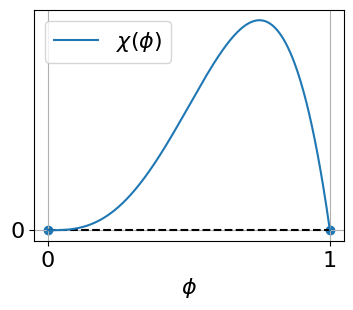
\includegraphics[width=0.8\textwidth]{pictures/equilibriums_case_1.png}
    \vspace{-0.3cm}
    \caption{Поведение функции $\chi(\phi)$, случай <<слабого напряжения>>.}
    \label{picture_equilibriums_case_1}
    \vspace{0.7cm}
    
    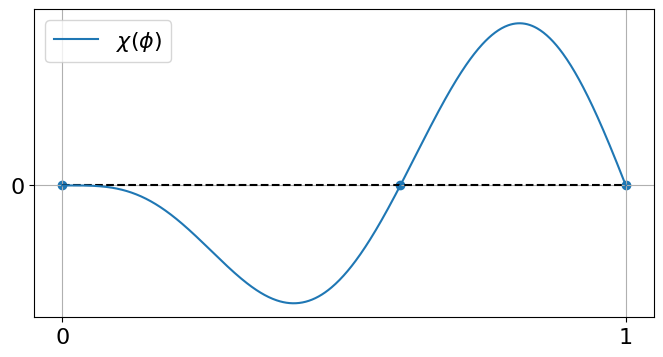
\includegraphics[width=0.8\textwidth]{pictures/equilibriums_case_2.png}
    \vspace{-0.3cm}
    \caption{Поведение функции $\chi(\phi)$, случай <<среднего непряжения>>.}
    \label{picture_equilibriums_case_2}
    \vspace{0.7cm}
    
    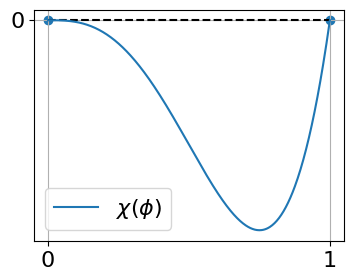
\includegraphics[width=0.8\textwidth]{pictures/equilibriums_case_3.png}
    \vspace{-0.3cm}
    \caption{Поведение функции $\chi(\phi)$, случай <<сильного напряжения>>.}
    \label{picture_equilibriums_case_3}
\end{figure}


\section{Разностная схема для одномерной задачи}
\label{section_scheme}

Будем численно решать задачу Коши в области $[0, w]_x \times [0, +\infty)_t$ для уравнения~\eqref{equation_one_dim_simpler} и граничных условий
\begin{equation}
    \phi(x, 0) = \phi_0(x); \quad \phi(0, t) = \phi_l(t); \quad \phi(w, t) = \phi_r(t) \text{.}
    \label{equation_cauchy_borders}
\end{equation}

Используем регулярную сетку с временным шагом $\tau$ и пространственным $h$. Пусть $n = w/h$ -- целое число. Пусть $(ah, b \tau)$ -- узлы сетки, $a = \overline{0, n}, \; b \in \mathbb{N}_0$. Обозначим $\phi_a^b$ значение сеточной функции $\phi$ в узле $(ah, b \tau)$. Перейдем к следующей разностной задаче:
\begin{equation}
    \cfrac{1}{m} \cfrac{\phi_a^{b + 1} - \phi_a^b}{\tau} = \cfrac{1}{2} K_\phi^2 \epsilon'(\phi_a^b) + \cfrac{\Gamma}{l^2} f'(\phi_a^b) + \cfrac{\Gamma}{2} \cfrac{\phi_{a + 1}^b - 2 \phi_a^b + \phi_{a - 1}^b}{h^2} \text{.}
    \label{equation_subtractive}
\end{equation}
Имеем четырехточечную явную разностную схему:
\begin{numcases}{}
    \mbox{$\begin{aligned}
        \phi_a^{b + 1} = \phi_a^b + m \tau \left( \cfrac{1}{2} K_\Phi^2 \epsilon'(\phi_a^b) + \cfrac{\Gamma}{l^2} f'(\phi_a^b) + \cfrac{\Gamma}{2} \cfrac{\phi_{a + 1}^b - 2 \phi_a^b + \phi_{a - 1}^b}{h^2} \right), \\ a = \overline{1, n - 1}, \quad b \in \mathbb{N} \text{;}
    \end{aligned}$}
    \label{scheme_transition} \\
    \phi_a^0 = \phi_0(ah); \quad \phi_0^b = \phi_l(b \tau); \quad \phi_n^b = \phi_r(b \tau) \text{.}
    \label{scheme_borders}
\end{numcases}

Легко видеть, что схема имеет первый порядок аппроксимации по времени и второй порядок аппроксимации по пространственной переменной $x$.

Получим необходимое условие устойчивости по принципу <<замороженных коэффициентов>> (см., например, \cite{bahvalov_computational_methods}). Пусть $\phi_a^b$ и $\phi_a^b + \delta_a^b$ -- решения разностного уравнения~\eqref{equation_subtractive}. Подставим в него $\phi_a^b + \delta_a^b$, получим:
\begin{multline*}
    \cfrac{1}{m} \cfrac{(\phi_a^{b + 1} + \delta_a^{b + 1}) - (\phi_a^b + \delta_a^b)}{\tau} = \cfrac{1}{2} K_\Phi^2 [\epsilon'(\phi_a^b) + \epsilon''(\phi_a^b) \delta_a^b + o(\delta_a^b)] + \\ + \cfrac{\Gamma}{l^2} [f'(\phi_a^b) + f''(\phi_a^b) \delta_a^b + o(\delta_a^b)] + \cfrac{\Gamma}{2} \cfrac{(\phi_{a + 1}^b + \delta_{a + 1}^b) - 2 (\phi_a^b + \delta_a^b) + (\phi_{a - 1}^b + \delta_{a - 1}^b)}{h^2} \text{.}
\end{multline*}
Линеаризуем по возмущению $\delta_a^b$ в точке $\phi_a^b = P$ и сократим слагаемые, учитывая, что $\phi_a^b$ есть решение разностной задачи:
\begin{equation}
    \delta_a^{b + 1} = \delta_a^b + m \tau \left( \cfrac{1}{2} K_\Phi^2 \epsilon''(P) \delta_a^b + \cfrac{\Gamma}{l^2} f''(P) \delta_a^b + \cfrac{\Gamma}{2} \cfrac{\delta_{a + 1}^b - 2 \delta_a^b + \delta_{a - 1}^b}{h^2} \right) \text{.}
    \label{equation_scheme_variation}
\end{equation} 

Применим спектральный признак устойчивости. Пусть $\delta_a^b = \lambda(\theta)^b \exp(\imath a \theta)$; подставим в уравнение \eqref{equation_scheme_variation} выражение для $\delta_a^b$ и, сократив на $\lambda(\theta)^b \exp(\imath a \theta)$, получим:
$$\lambda(\theta) = 1 + m \tau \left( \cfrac{1}{2} K_\Phi^2 \epsilon''(P) + \cfrac{\Gamma}{l^2} f''(P) + \cfrac{\Gamma}{2} \cfrac{e^{i \theta} - 2 + e^{-i \theta}}{h^2} \right) \text{,}$$
или
\begin{equation}
    \lambda(\theta) = 1 + m \tau \left( \cfrac{1}{2} K_\Phi^2 \epsilon''(P) + \cfrac{\Gamma}{l^2} f''(P) - \cfrac{2 \Gamma}{h^2} \sin^2 \cfrac{\theta}{2} \right) \text{.}
    \label{equation_spectral}
\end{equation}

Согласно спектральному признаку, связь $\tau = \tau(h)$ дает устойчивые вычисления в области $[0, w]_x \times [0, T]_t$ при $\tau, h \to 0$, если существует $C > 0$, такое что для любого~$\theta$ выполнено $|\lambda(\theta)| \leqslant e^{C\tau}$. Заметим, что можно использовать условие $|\lambda(\theta)| \leqslant 1 + C\tau$, как более сильное. Если же для любого $\theta$ выполнено $|\lambda(\theta)| \leqslant 1$, то устойчивыми будут вычисления в области $[0, w]_x \times [0, +\infty)_t$ с бесконечным временным интервалом. Строго говоря, условие спектрального метода необходимое, но не достаточное для устойчивости разностной схемы. Однако на практике устойчивость следует ожидать.

Для начала рассмотрим выражение \eqref{equation_spectral} в точке $P = 0$. Имеем $f''(0) = 0, \; \epsilon''(0) \hm = 0$. Уравнение \eqref{equation_spectral} принимает вид
$$\lambda(\theta) = 1 - \cfrac{2 \tau m \Gamma}{h^2} \sin^2 \cfrac{\theta}{2} \text{.}$$
Значит, для любого $\theta$ выполнено $|\lambda(\theta)| \leqslant 1$, если и только если
\begin{equation}
     \tau \leqslant \cfrac{h^2}{m \Gamma} \text{.}
     \label{condition_spectral_0}
\end{equation}
При выполнении условия \eqref{condition_spectral_0} следует ожидать устойчивый расчет при полностью разрушенной или близкой к таковой среде ($\phi \approx 0$) в области $[0, w]_x \times [0, +\infty)_t$ с бесконечным временным интервалом.

Заметим, что при условии \eqref{condition_spectral_0} к тому же ожидается устойчивый расчет на множестве $[0, w]_x \times [0, T]_t$ при любом $\phi$. В этом случае справедливо неравенство
$$|\lambda(\theta)| \leqslant 1 + m \tau \left| \cfrac{1}{2} K_\Phi^2 \epsilon''(P) + \cfrac{\Gamma}{l^2} f''(P) \right| \text{.}$$
Значит, для некоторого $C$ верно $|\lambda(\theta)| \leqslant 1 + C \tau$, так как $\epsilon''(\phi)$ и $f''(\phi)$ -- непрерывные на отрезке $[0, 1]$ функции. Следует отметить, что, несмотря на подобную универсальность, оценка \eqref{condition_spectral_0} плохо применима на практике и нуждается в уточнении, которое будет сделано позже.

Теперь рассмотрим выражение \eqref{equation_spectral} в точке $P = 1$. Имеем $f''(1) < 0, \; \epsilon''(1) > 0$. Заметим, что при $(K_\Phi^2/2) \epsilon''(1) + (\Gamma/l^2) f''(1) \leqslant 0$ можно добиться $|\lambda(\theta)| \leqslant 1$, потребовав, подобно условию \eqref{condition_spectral_0}, $\tau \leqslant h^2/(2m \Gamma)$ и притом достаточно малое $\tau$. Если подставить в упомянутое неравенство значения $f''(1) = -12, \; \epsilon''(1) = 12 \epsilon_0/(1 + \delta)^2$ (см. выражение~\eqref{equation_epsilon_phi_phi}), то оно преобразуется в
\begin{equation}
    \cfrac{K_\Phi^2 l^2 \epsilon_0}{2 \Gamma (1 + \delta)^2} \leqslant 1 \text{.}
    \label{condition_spectral_possible_1}
\end{equation}

Итак, при условии \eqref{condition_spectral_possible_1} ожидается существование таких $\tau$ и $h$, что расчет устойчив при $\phi \approx 1$ на множестве с бесконечным временным интервалом. Закономерно, что условие \eqref{condition_spectral_possible_1} эквивалентно условию \eqref{condition_equilibrium_1_stable} устойчивости положения равновесия $\phi \equiv 1$ уравнения \eqref{equation_one_dim_simpler}.


\section{Численное исследование}
\label{section_computational_analysis}

\subsection{Улучшенная оценка устойчивости}

В предыдущем разделе из анализа уравнения \eqref{equation_spectral} было получено условие \eqref{condition_spectral_0}, необходимое для устойчивости разностной схемы \eqref{scheme_transition}, \eqref{scheme_borders} при $\phi \approx 0$. Предположение о его полезности основано на том, что типичным поведением модели будет некоторый процесс перехода $\phi$ от $1$ к $0$ (<<разрушение>>) за конечное время, а затем бесконечно долгое пребывание в состоянии $\phi \approx 0$.

Однако проделанного анализа уравнения \eqref{equation_spectral} в точке $\phi = 0$ недостаточно. В самом деле, было использовано, что $\epsilon''(0) = 0$ (см. выражение \eqref{equation_epsilon_phi_phi}), но не учтено, что $\epsilon''(\phi)$ при малых $\delta$ вблизи $0$ растет очень быстро и достигает больших значений (рис.~\ref{picture_eps_phi_phi}). Получается, что модель, устойчивая в точке $0$, может работать неадекватно в малой ее окрестности. Это нас, конечно, не устраивает -- улучшим оценку устойчивости.

\begin{figure}[!tp]
    \centering
    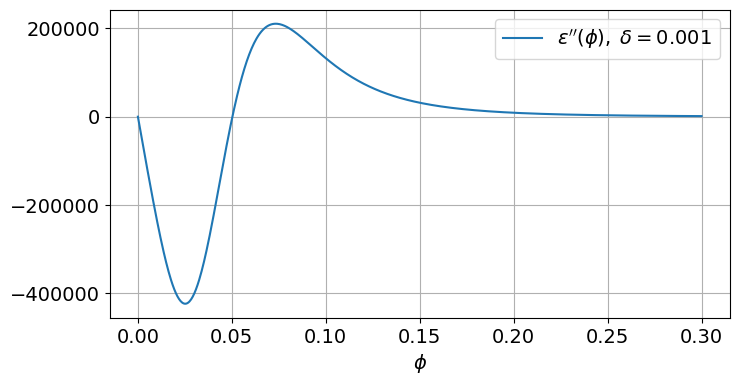
\includegraphics[width=\textwidth]{pictures/eps_phi_phi.png}
    \vspace{-0.7cm}
    \caption{Поведение функции $\epsilon''(\phi)$ около $0$.}
    \label{picture_eps_phi_phi}
\end{figure}

Нужно оценить экстремумы функции $\epsilon''(\phi)$ вблизи $0$. Для начала найдем нули $\epsilon'''(\phi)$. Имеем:
$$f'''(\phi) = 24 - 72 \phi; \quad \epsilon'''_{fff} = \cfrac{-6 \epsilon_0}{(f(\phi) + \delta)^4} \text{;}$$
\begin{equation}
    \epsilon''' = \epsilon'''_{fff} \cdot (f')^3 + 3 \epsilon''_{ff} \cdot f' \cdot f'' + \epsilon'_f \cdot f''' = \epsilon_0 \cfrac{-6 (f')^3 + 6 (f + \delta) f' f'' - (f + \delta)^2 f'''}{(f + \delta)^4} \text{.}
    \label{equation_epsilon_phi_phi_phi}
\end{equation}
Приравняв $\epsilon'''$ к $0$, получим:
$$-6 (f')^3 + 6 (f + \delta) f' f'' - (f + \delta)^2 f''' = 0 \text{,}$$
или
\begin{multline*}
    -6(12 \phi^2 (1 - \phi))^3 + 6(4 \phi^3 - 3\phi^4 + \delta) \cdot 12 \phi^2 (1 - \phi) \cdot 12 \phi (2 - 3\phi) - \\ - (4 \phi^3 - 3 \phi^4 + \delta)^2 \cdot 24 (1 - 3 \phi) = 0 \text{.}
\end{multline*}
Разделим последнее уравнение на $24\phi^6$, получим:
$$-3 \cdot 12^2 (1 - \phi)^3 + 36 \left(4 - 3\phi + \cfrac{\delta}{\phi^3} \right)(1 - \phi)(2 - 3\phi) - \left(4 - 3 \phi + \cfrac{\delta}{\phi^3} \right)^2 (1 - 3 \phi) = 0 \text{.}$$
Пусть $\delta_n \to +0$ и корень $\phi_n \to +0$, причем $\delta_n/\phi_n^3$ ограничено. Тогда:
$$-3 \cdot 12^2 \cdot 1^3 + 36 \left(4 + \cfrac{\delta_n}{\phi_n^3} \right) \cdot 1 \cdot 2 - \left(4 + \cfrac{\delta_n}{\phi_n^3} \right)^2 \cdot 1 \to 0 \text{,}$$
$$\left(4 + \cfrac{\delta_n}{\phi_n^3} \right)^2 - 72 \left(4 + \cfrac{\delta_n}{\phi_n^3} \right) + 3 \cdot 12^2 \to 0 \text{.}$$
Значит, последовательность $4 + \delta_n/\phi_n^3$ имеет не более двух частичных пределов $\xi_+$ и $\xi_-$ -- корней уравнения $\xi^2 - 72 \xi + 432 = 0$. Первому корню $\xi_+ = 36 + 12 \sqrt{6}$ соответствует
$$\phi = \cfrac{1}{\sqrt[3]{32 + 12 \sqrt{6}}} \sqrt[3]{\delta_n} \approx \cfrac{1}{3.945} \sqrt[3]{\delta_n} \text{,}$$
второму корню $\xi_- = 36 - 12 \sqrt{6}$ соответствует
$$\phi = \cfrac{1}{\sqrt[3]{32 - 12 \sqrt{6}}} \sqrt[3]{\delta_n} \approx \cfrac{1}{1.376} \sqrt[3]{\delta_n} \text{.}$$

Из проделанного рассуждения следует, что при $\delta \to +0$ функция $\epsilon'''(\phi)$ имеет в окрестности $0$ два корня
\begin{equation}
    \phi_{\pm} = \cfrac{1}{\sqrt[3]{32 \pm 12 \sqrt{6}}} \sqrt[3]{\delta} [1 + o(1)] \text{.}
    \label{equation_epsilon_phi_phi_phi_roots}
\end{equation}

Оценим $\epsilon''(\phi)$ в точках $\phi_{\pm}$ при $\delta \to +0$. Пусть $\phi = (1/c) \sqrt[3]{\delta}, \; c \in \mathbb{R}$. Тогда:
\begin{multline*}
    \cfrac{\epsilon''}{\epsilon_0} = \cfrac{2(f')^2 - (f + \delta)f''}{(f + \delta)^3} = \cfrac{2 \cdot 12^2 \phi^4 (1 - \phi)^2 - (4 \phi^3 - 3 \phi^4 + \delta) \cdot 12 \phi (2 - 3 \phi)}{(4 \phi^3 - 3 \phi^4 + \delta)^3} = \\ = \cfrac{2 \cdot 12^2 - 8 \cdot 12 - 24 (\delta/\phi^3)}{4^3 + 3 \cdot 4^3 (\delta/\phi^3) + 3 \cdot 4 (\delta/\phi^3)^2 + (\delta/\phi^3)^3} \cdot \cfrac{1}{\phi^5}[1 + o(1)] = c^5 \delta^{-5/3} \cfrac{24(8 - c^3)}{(4 + c^3)^3}[1 + o(1)] \text{.}
\end{multline*}
Отсюда:
\begin{equation}
    \epsilon''(\phi_+) \approx -4.378 \epsilon_0 \delta^{-5/3}; \quad \epsilon''(\phi_-) \approx 2.216 \epsilon_0 \delta^{-5/3} \text{.}
    \label{value_epsilon_phi_phi_bounds}
\end{equation}
Оценки экстремумов $\epsilon''(\phi)$ вблизи $0$ показаны на рис. \ref{picture_eps_phi_phi_multiplied}.

\begin{figure}[!tp]
    \centering
    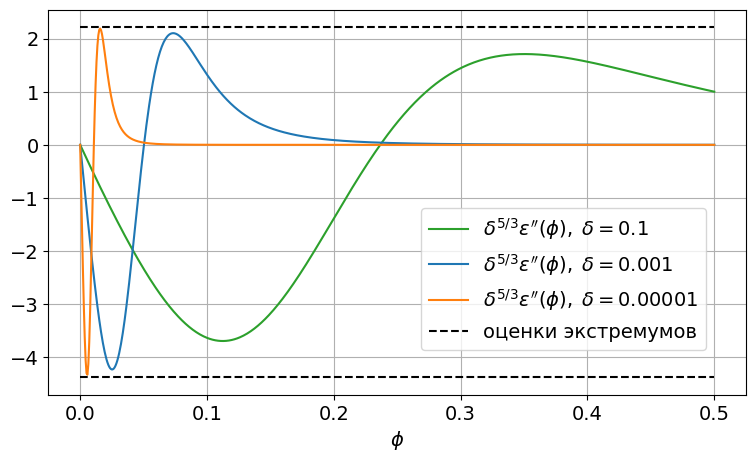
\includegraphics[width=\textwidth]{pictures/eps_phi_phi_multiplied.png}
    \caption{Сравнение функций $\delta^{5/3} \epsilon''(\phi)$ при различных значениях $\delta$.}
    \label{picture_eps_phi_phi_multiplied}
\end{figure}

Получим новую оценку устойчивости, рассмотрев уравнение \eqref{equation_spectral} в точке $\phi = \phi_+$. $\epsilon''(\phi_+) \approx -4.4 \epsilon_0 \delta^{-5/3}$. Сумма в скобках отрицательна ($\delta$ мало, $\epsilon''(\phi_+)$ велико по модулю и отрицательно), поэтому $f''(\phi_0) > 0$ можно считать равным $0$: оценку это только усилит. Преобразовав уравнение \eqref{equation_spectral}, получим:
$$\lambda(\theta) = 1 + m \tau \left( -\cfrac{2.2 K_\Phi^2 \epsilon_0}{\delta^{5/3}} - \cfrac{2 \Gamma}{h^2} \sin^2 \cfrac{\theta}{2} \right) \text{.}$$
Условие $|\lambda(\theta)| \leqslant 1$ справедливо для любого $\theta$, если и только если
\begin{equation}
    \tau \leqslant \left( \cfrac{1.1 m K_\Phi^2 \epsilon_0}{\delta^{5/3}} + \cfrac{m \Gamma}{h^2} \right)^{-1} \text{.}
    \label{condition_spectral_better_theoretical}
\end{equation}

Для применения на практике оценку \eqref{condition_spectral_better_theoretical} нужно брать <<с запасом>> (экспериментальное обоснование будет дано позже). Сделаем оценку строже, примерно удвоив знаменатель:
\begin{equation}
    \tau \leqslant \cfrac{1}{2m} \left( \cfrac{K_\Phi^2 \epsilon_0}{\delta^{5/3}} + \cfrac{\Gamma}{h^2} \right)^{-1} \text{.}
    \label{condition_spectral_better}
\end{equation}

Более простая оценка не слабее оценки \eqref{condition_spectral_better} выглядит следующим образом:
\begin{equation}
    \tau \leqslant \cfrac{1}{2m} \min \left(\cfrac{\delta^{5/3}}{K_\Phi^2 \epsilon_0}, \; \cfrac{h^2}{\Gamma} \right) \text{.}
    \label{condition_spectral_better_simpler}
\end{equation}

Полученная оценка \eqref{condition_spectral_better} устойчивости разностной схемы \eqref{scheme_transition}, \eqref{scheme_borders} содержит все параметры уравнения \eqref{equation_one_dim_simpler}, кроме $l$.


\subsection{Вычислительный эксперимент: устойчивость}

Была написана программа, реализующая разностную схему \eqref{scheme_transition}, \eqref{scheme_borders}. Проверим на практике устойчивость и сходимость.

Зафиксируем параметры уравнения \eqref{equation_one_dim_simpler}:
\begin{equation}
    \epsilon_0 = 0.2, \; \delta = 0.04, \; l = 1.0, \; \Gamma = 1.0, \; m = 0.5, \; K_\Phi = 4.8 \text{.}
    \label{experiment_parameters}
\end{equation}
Отметим, что перед нами случай <<сильного напряжения>> (см. выражение \eqref{characteristic_equilibriums}).

Моделируем решение в области 
\begin{equation}
    \Omega = [0, w]_x \times [0, T]_t, \; w = 5, \; T = 1 \text{.}
    \label{experiment_set}
\end{equation}

Зададим следующие краевые условия:
\begin{equation}
\begin{gathered}
    \phi(0, t) = 1, \; \phi(w, t) = 1 \text{,} \\
    \phi(x, 0) \equiv \phi_0(x) = \begin{cases}
        1, \; \text{если} \; x \leqslant 2.25 \; \text{или} \; x \geqslant 2.75 \text{;} \\
        1 - 0.025 \cdot [1 + \cos(4 \pi x)], \; \text{если} \; 2.25 < x < 2.75 \text{.}
    \end{cases}
\end{gathered} \label{experiment_borders}
\end{equation}
Обратим внимание, что $\phi_0(x)$ дважды дифференцируема всюду, кроме конечного числа точек, с ограниченной второй производной.

Обозначим $n_x$ количество отрезков разбиения $[0, w]_x$ (узлов, соответственно, $n_x \hm + 1$); $n_t$ -- количество отрезков разбиения $[0, T]_t$. $h = w/n_x, \; \tau = T/n_t$.

\begin{figure}[!tp]
    \centering
    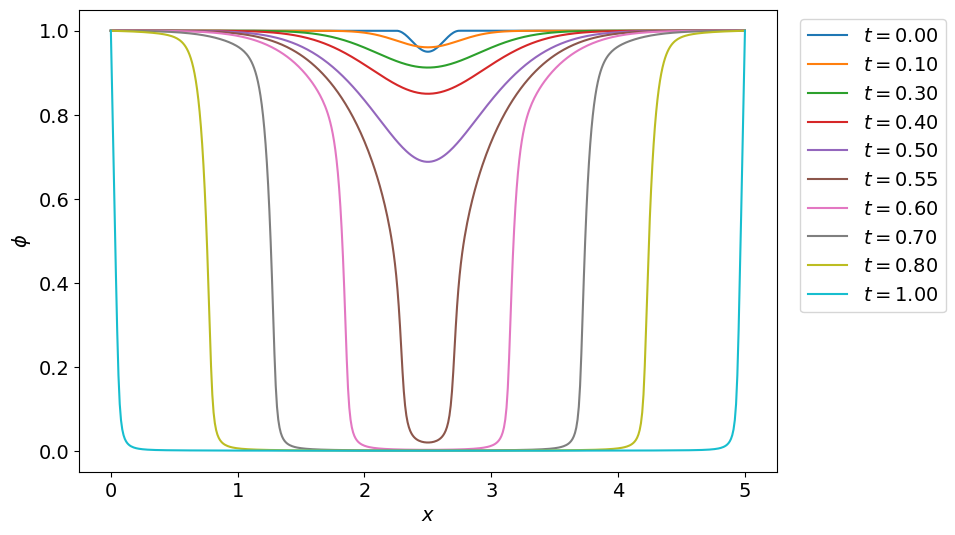
\includegraphics[width=\textwidth]{pictures/typical_solution.png}
    \vspace{-0.8cm}
    \caption{Типичное решение задачи, $n_x = 10^3, \; n_t = 10^5$.}
    \label{picture_typical_solution}
\end{figure}

Для начала посмотрим на типичное решение исследуемой задачи (рис. \ref{picture_typical_solution}). Видно постепенное развитие канала электрического пробоя (разрушение среды) из небольшого начального возмущения фазового поля $\phi$ неповрежденной среды. Примерно в момент времени $t = 0.55$ канал пробоя <<прорастает насквозь>>, а именно, $\phi$ вблизи точки $x = 2.5$ приближается к нулевому значению. Обратим внимание, что в период времени $t \hm \in (0.3, \; 0.55)$ канал пробоя (область, где $\phi$ существенно отличается от $1$) практически не растет в ширину, а при $t > 0.55$, напротив, растет в ширину почти с постоянной скоростью.

Проверим полученную в предыдущем разделе оценку \eqref{condition_spectral_better} устойчивости разностной схемы. Будем считать, что в вычислительном эксперименте схема неустойчива, если программа завершилась с ошибкой: произошло деление на $0$ (в формуле \eqref{equation_epsilon} функции $\epsilon(\phi)$ при $f(\phi) = -\delta$) или значения $\phi$ ушли на бесконечность (переполнился тип double). Будем перебирать $n_x$ и $n_t$, запоминая пары соседних точек, в одной из которых устойчивость есть, а в другой нет. Так получим опытную оценку устойчивости схемы. Отобразим ее на графике вместе с оценкой \eqref{condition_spectral_better} (рис. \ref{picture_stability_bounds}).

Эксперимент показывает, что оценка \eqref{condition_spectral_better} удачна: она примерно повторяет контур опытной оценки, к тому же ее график лежит выше, то есть она имеет некоторый <<запас>> до момента, когда в программе возникает ошибка. Именно ради этого <<запаса>> знаменатель исходной оценки  \eqref{condition_spectral_better_theoretical} был удвоен.

\begin{figure}[!tp]
    \centering
    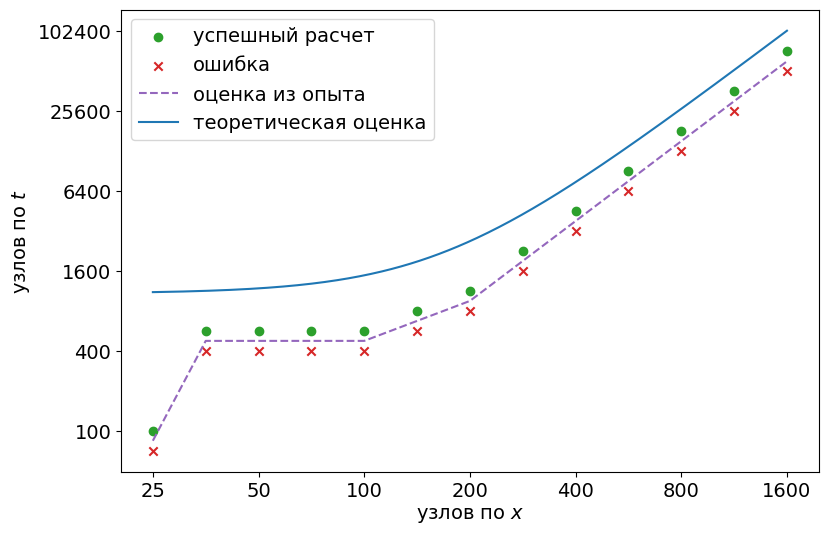
\includegraphics[width=\textwidth]{pictures/stability_bounds.png}
    \vspace{-0.7cm}
    \caption{Теоретическая и опытная оценки устойчивости разностной схемы.}
    \label{picture_stability_bounds}
\end{figure}


\subsection{О сходимости решения разностной задачи}

Если разностная схема аппроксимирует задачу Коши и к тому же обладает устойчивостью при заданной связи $\tau =\tau(h)$, то решение разностной задачи сходится к решению задачи Коши при $h \to 0$.

Расшифруем перечисленные понятия более формально.

Пусть $\Omega \subset \mathbb{R}^s$ -- пространство независимых переменных, $\Gamma = \partial \Omega$ -- граница $\Omega$, $\Int \Omega = \Omega \smallsetminus \partial \Omega$ -- внутренность $\Omega$; задан класс $Y$ функций $y(\mathbf{x})$ на $\Omega$ (обладающих некоторыми содержательными свойствами, например, гладкостью).

Задан оператор $R: Y \longrightarrow I$, где $I$ -- некоторое пространство функций на $\Int \Omega$; задан оператор $r: Y \longrightarrow G$, где $G$ -- некоторое пространство функций на $\partial \Omega$. $R$ и $r$ не обязательно линейные; подразумевается, что они включают в себя операции дифференцирования. Сформулируем дифференциальную задачу:
\begin{equation}
    \{ \quad Ry = 0; \quad ry = 0 \quad \} \text{.}
    \label{equation_formal_differential}
\end{equation}
Здесь $y(\mathbf{x}) \in Y$ -- искомая функция. Первое уравнение имеет смысл условия на $y$ во внутренности $\Omega$, второе -- краевого условия.

В пространстве $\Omega$ введем сетку, то есть определим некоторое конечное подмножество $\Omega_h \subset \Omega$. Здесь $h$ -- параметр, имеющий смысл мелкости шага сетки, -- то есть, строго говоря, определено семейство сеток. Функцию $y \in Y$ можно ограничить на $\Omega_h$ -- введем обозначение $[y]_h = y|_{\Omega_h}$. Пусть $Y_h = \{[y]_h: y \in Y\}, \; I_h = \{[i]_h: i \in I\}, \; G_h \hm = \{[g]_h: g \in G\}$. Некоторые $R_h: Y_h \longrightarrow I_h$ и $r_h: Y_h \longrightarrow G_h$ будем называть разностными операторами. Теперь можно сформулировать разностную задачу:
\begin{equation}
    \{ \quad R_h y_h = 0; \quad r_h y_h = 0 \quad \} \text{.}
    \label{equation_formal_subtractive}
\end{equation}
$y_h \in Y_h$ -- искомая сеточная функция.

Пусть на пространствах $Y$, $I$, $G$ определены некоторые нормы $\| \cdot \|_Y$, $\| \cdot \|_I$, $\| \cdot \|_G$ соответственно. Пусть на пространстве $Y_h$ определена норма $\| \cdot \|_{Y_h}$, такая что $\forall y \in Y \; \| \, [y]_h \, \|_{Y_h} \to \| \, y \, \|_Y$ при $h \to 0$. В этом случае нормы $\| \cdot \|_Y$ и $\| \cdot \|_{Y_h}$ назовем \emph{согласованными}. Пусть аналогично $\| \cdot \|_{I_h}$ и $\| \cdot \|_{G_h}$ -- нормы на $I_h$ и $G_h$, согласованные с $\| \cdot \|_I$ и $\| \cdot \|_G$ соответственно.

Теперь можно формально определить аппроксимацию, устойчивость и сходимость.

Разностная задача \eqref{equation_formal_subtractive} \emph{аппроксимирует} дифференциальную задачу \eqref{equation_formal_differential}, если
$$\forall y \in Y \quad \| \, [Ry]_h - R_h [y]_h \, \|_{I_h} + \| \, [ry]_h - r_h [y]_h \, \|_{G_h} \to 0 \text{ при } h \to 0 \text{.}$$
Порядок $k$ стремления выражения к $0$ по $h$ называют порядком аппроксимации.

Решение $y_h$ разностной задачи \eqref{equation_formal_subtractive} \emph{сходится} к решению $y$ дифференциальной задачи \eqref{equation_formal_differential}, если
$$\| \, [y]_h - y_h \, \|_{Y_h} \to 0 \text{ при } h \to 0 \text{.}$$
Порядок $k$ стремления выражения к $0$ по $h$ называют порядком сходимости.

Разностная задача \eqref{equation_formal_subtractive} \emph{устойчива}, если
$$\exists M \in \mathbb{R} \; \forall h \; \forall y_h, z_h \in Y_h \quad \| \, y_h - z_h \, \|_{Y_h} \leqslant M \cdot (\| \, R_h y_h - R_h z_h \, \|_{I_h} + \| \, r_h y_h - r_h z_h \, \|_{G_h}) \text{.}$$

Легко видеть, что из аппроксимации и устойчивости следует сходимость. Пусть $y$ -- решение задачи \eqref{equation_formal_differential}, $y_h$ -- решение задачи \eqref{equation_formal_subtractive}. Запишем неравенство из определения устойчивости, положив $z_h = [y]_h$:
$$\| \, y_h - [y]_h \, \|_{Y_h} \leqslant M \cdot (\| \, R_h y_h - R_h [y]_h \, \|_{I_h} + \| \, r_h y_h - r_h [y]_h \, \|_{G_h}) \text{.}$$
$y_h$ -- решение разностной задачи, следовательно, $R_h y_h \equiv 0, \; r_h y_h \equiv 0$. $y$ -- решение дифференциальной задачи, $Ry \equiv 0, \; ry \equiv 0$, а значит, $[Ry]_h \equiv 0, \; [ry]_h \equiv 0$. Вычтя и прибавив нулевые слагаемые, получим:
$$\| \, y_h - [y]_h \, \|_{Y_h} \leqslant M \cdot (\| \, [Ry]_h - R_h [y]_h \, \|_{I_h} + \| \, [ry]_h - r_h [y]_h \, \|_{G_h}) \text{.}$$
В правой части неравенства выражение из определения аппроксимации, стремящееся к~$0$. В итоге $\| \, [y]_h - y_h \, \|_{Y_h} \to 0$ -- доказана сходимость. Отметим, что порядок сходимости $k$ в таком случае совпадает с порядком аппроксимации.

Приведенные построения могут быть непосредственно применены к разностной схеме, описанной в разделе \ref{section_scheme}, тем самым доказывая ее сходимость.


\subsection{Вычислительный эксперимент: сходимость}

Аппроксимация схемой \eqref{scheme_transition}, \eqref{scheme_borders} задачи Коши \eqref{equation_one_dim_simpler}, \eqref{equation_cauchy_borders} очевидна; для устойчивости схемы получено условие \eqref{condition_spectral_better}, строго говоря, являющееся лишь необходимым, но применимое на практике. Теперь экспериментально проверим сходимость.

Поясним связь формальных конструкций предыдущего раздела с решаемой задачей Коши.

На множестве $C_2(\Omega)$ дважды непрерывно дифференцируемых функций в замкнутой области $\Omega = [0, w]_x \times [0, T]_t$ рассмотрим следующие нормы: непрерывную $\| \cdot \|_C$ и $L_2$-норму $\| \cdot \|_2$.
$$\| \, f \, \|_C = \max\limits_{(x, t) \in \Omega} f(x, t); \qquad \| \, f \, \|_{2} = \sqrt{\int\limits_{\Omega} f^2(x, t) dx dt} \text{.}$$
Эти же нормы введем на множествах $C(\partial \Omega)$ и $C(\Int \Omega)$ непрерывных функций на границе и внутренности $\Omega$ соответственно.

Теперь рассмотрим регулярную сетку $\Omega_{h, \tau}$; введем некоторую зависимость $\tau \hm = \tau(h)$. Ограничивая функции из $C_2(\Omega)$, $C(\Int \Omega)$ и $C(\partial \Omega)$ на множестве $\Omega_h = \Omega_{h, \tau(h)}$, получаем множества $C_2(\Omega)_h$, $C(\Int \Omega)_h$ и $C(\partial \Omega)_h$ сеточных функций.

На перечисленных множествах сеточных функций введем нормы, согласованные с $\| \cdot \|_C$ и $\| \cdot \|_2$:
$$\| \, f_a^b \, \|_C = \max\limits_{(a, b) \in \Omega_h} f_a^b; \qquad \| \, f_a^b \, \|_2 = \sqrt{\cfrac{1}{h \tau}\sum\limits_{(a, b) \in \Omega_h} (f_a^b)^2} \text{.}$$

Задачу Коши \eqref{equation_one_dim_simpler}, \eqref{equation_cauchy_borders} легко привести к виду \eqref{equation_formal_differential}, где $R: C_2(\Omega) \longrightarrow C(\Int \Omega)$, $r: C_2(\Omega) \longrightarrow C(\partial \Omega)$; разностную задачу \eqref{scheme_transition}, \eqref{scheme_borders} -- к виду \eqref{equation_formal_subtractive}, где $R_h: C_2(\Omega)_h \hm \longrightarrow C(\Int \Omega)_h$, $r_h: C_2(\Omega)_h \longrightarrow C(\partial \Omega)_h$.

Перейдем к вычислительному эксперименту. Сходимость будем проверять по описанным выше нормам $\| \cdot \|_C$ и $\| \cdot \|_2$ на множестве сеточных функций. Так как аналитическое решение задачи Коши не известно, будем сравнивать ряд результатов на все более мелких сетках по норме с лучшим результатом в ряду. При сравнении функцию на более мелкой сетке ограничиваем на более крупной, игнорируя часть узлов.

Зафиксируем ранее использовавшиеся параметры уравнения \eqref{experiment_parameters}, \eqref{experiment_set}; зададим краевые условия \eqref{experiment_borders}. Положим $n_x = w / h$ -- число отрезков разбиения по $x$, $n_t = T / \tau$ -- по $t$.

Во всех описанных далее вариантах расчетов соблюдается условие устойчивости~\eqref{condition_spectral_better}.

Для начала зафиксируем $n_x = 200$ и будем перебирать $n_t$, каждый раз увеличивая его вдвое. Сравнение по нормам с результатом при $n_t = 204800$ изображено на рис. \ref{picture_convergence_fixed_nx}. Разностная схема имеет первый порядок аппроксимации по $t$; опыт показывает первый порядок сходимости ошибки $O(\tau)$.

Зафиксируем $n_t = 204800$ и будем перебирать $n_x$, каждый раз увеличивая его вдвое. Сравнение по нормам с результатом при $n_x = 1600$ изображено на рис. \ref{picture_convergence_fixed_nt}. Разностная схема имеет второй порядок аппроксимации по $x$; опыт показывает второй порядок сходимости ошибки $O(h^2)$.

\begin{figure}[!tp]
    \centering
    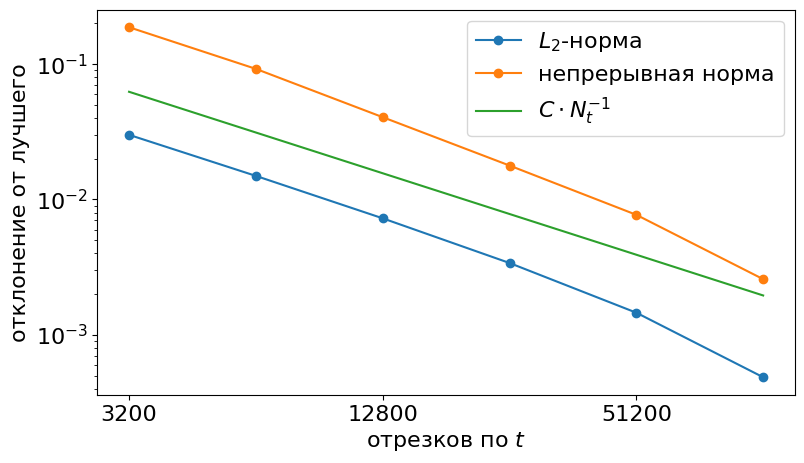
\includegraphics[width=0.75\textwidth]{pictures/convergence_fixed_nx.png}
    \vspace{-0.2cm}
    \caption{Ошибка решения по норме при фиксированном $n_x = 200$.}
    \label{picture_convergence_fixed_nx}
    \vspace{0.7cm}
    
    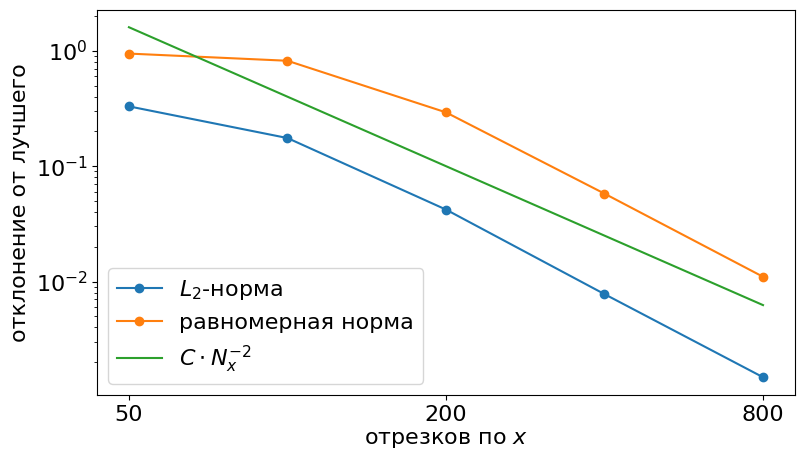
\includegraphics[width=0.75\textwidth]{pictures/convergence_fixed_nt.png}
    \vspace{-0.2cm}
    \caption{Ошибка решения по норме при фиксированном $n_t = 204800$.}
    \label{picture_convergence_fixed_nt}
    \vspace{0.7cm}
    
    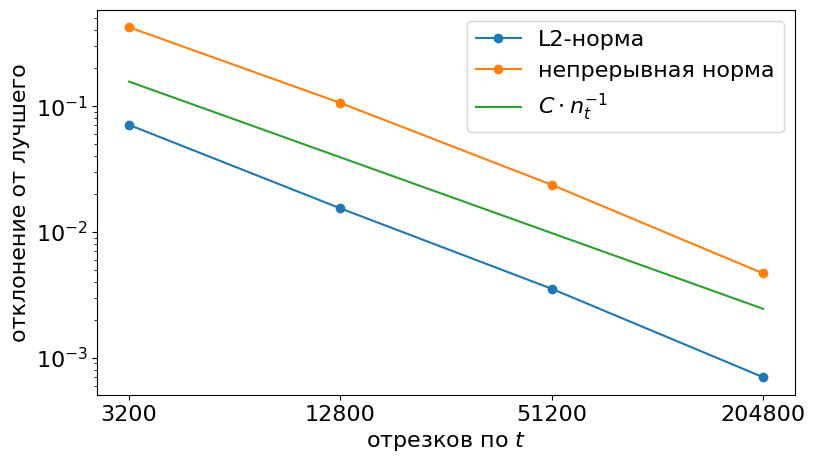
\includegraphics[width=0.75\textwidth]{pictures/convergence_connected.png}
    \vspace{-0.2cm}
    \caption{Ошибка решения по норме при $n_t = 0.08 \cdot n_x^2$.}
    \label{picture_convergence_connected}
\end{figure}

Теперь свяжем $n_x$ и $n_t$ уравнением, так чтобы при $h, \tau \to 0$ выполнялось условие устойчивости \eqref{condition_spectral_better}. При выбранных параметрах модели подойдет $n_t = 0.08 \cdot n_x^2$. Аналогично проведем сравнение ряда измерений по норме с лучшим (рис. \ref{picture_convergence_connected}). Как и ожидалось, измерения показывают сходимость $O(\tau + h^2) = O(\tau)$ первого порядка по времени при выбранном уравнении связи.

В первых двух опытах, без стремления обоих шагов сетки к $0$, последовательности сеточных функций имели неясный предел. В третьем же, если принять предположение об устойчивости разностной схемы, сеточные функции сходятся к решению задачи Коши \eqref{equation_one_dim_simpler}, \eqref{equation_cauchy_borders}.

\pagebreak


\subsection{Вычислительный эксперимент: положения равновесия}

Ранее были исследованы положения равновесия уравнения \eqref{equation_one_dim_simpler} вида $\phi \equiv C$. Их количество и устойчивость определяется значением выражения \eqref{characteristic_equilibriums} (обозначено $\xi$). Проверим этот результат экспериментально.

Зададим модели параметры \eqref{experiment_parameters}, \eqref{experiment_set}. В качестве начального условия берем возмущенное положение равновесия: $\phi(x, 0) = C + A \cos(\omega x); \; \phi(0, t) \equiv \phi(0, 0), \; \phi(w, t) \hm \equiv \phi(w, 0)$. Амплитуда $A$ мала, порядка $0.01$. $n_x = 800, \; n_t = 51200$.

Если положение равновесия устойчиво, то при любом $\omega$ возмущение угасает; если неустойчиво, то существует некоторое $\omega_0$, такое что при $\omega < \omega_0$ возмущение растет.

Положим $K_{\Phi, 1} = 0, \; K_{\Phi, 2} = 1.1, \; K_{\Phi, 3} = 4.8$. Как было сказано выше, $\delta = 0.04$. В таком случае $\xi_1 = 0 < \delta^2, \; \xi_2 = 0.121 \in (\delta^2, (1 + \delta)^2), \; \xi_3 = 2.304 > (1 + \delta)^2$.

Вначале рассмотрим $K_{\Phi, 1} = 0, \; \xi_1 < \delta^2$ -- случай слабого электрического напряжения. Система имеет два положения равновесия: $\phi \equiv 0$ неустойчивое, $\phi \equiv 1$ устойчивое. На рис. \ref{picture_equilibrium_1_0}, \ref{picture_equilibrium_1_1} видно теоретически предсказанное поведение возмущенной среды: при $C = 0$ возмущение растет, при $C = 1$ -- затухает. В точке $C = 0$ производная функции $\chi(\phi)$ (см. выражение \eqref{equation_equilibruim_characteristic}) равна $0$, поэтому, чтобы увидеть рост возмущения, приходится брать небольшое $\omega$, обеспечивая небольшое значение $\partial^2 \phi / \partial x^2$. В эксперименте с $\phi \equiv 1$ взято $C = 1 - A$, чтобы значения $\phi$ не превосходили $1$.

\begin{figure}[!t]
    \centering
    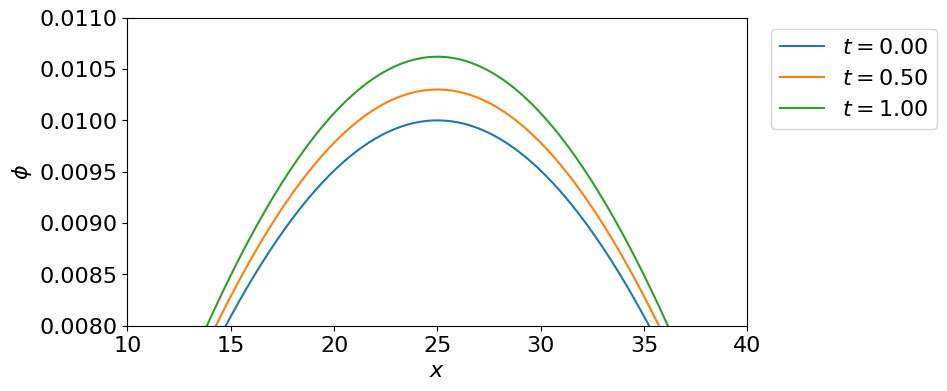
\includegraphics[width=\textwidth]{pictures/equilibrium_1_0.png}
    \vspace{-0.8cm}
    \caption{Случай слабого напряжения: возмущенное положение равновесия $\phi \equiv 0$, \linebreak неустойчивое.}
    \label{picture_equilibrium_1_0}
    \vspace{0.5cm}
    
    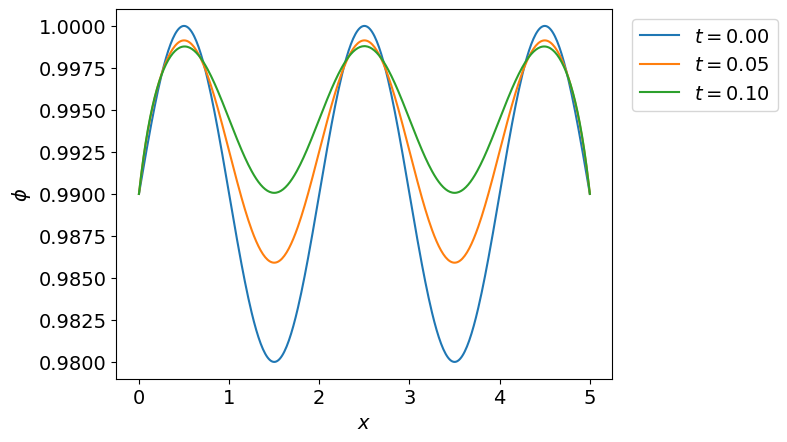
\includegraphics[width=\textwidth]{pictures/equilibrium_1_1.png}
    \vspace{-0.8cm}
    \caption{Случай слабого напряжения: возмущенное положение равновесия $\phi \equiv 1$, \linebreak устойчивое.}
    \label{picture_equilibrium_1_1}
\end{figure}

Теперь рассмотрим $K_{\Phi, 2} = 1.1, \; \xi_2 \in (\delta^2, (1 + \delta)^2)$ -- случай среднего напряжения. Система имеет три положения равновесия: $\phi \equiv 0$ устойчивое, $\phi \equiv C_3 \approx 0.5$ неустойчивое ($C_3$ -- корень функции $\chi(\phi)$ в интервале $(0, 1)$), $\phi \equiv 1$ устойчивое. Поведение возмущенной среды изображено на рис. \ref{picture_equilibrium_2_0}, \ref{picture_equilibrium_2_05}, \ref{picture_equilibrium_2_1}, оно соответствует теоретическим результатам.

\begin{figure}[!tp]
    \centering
    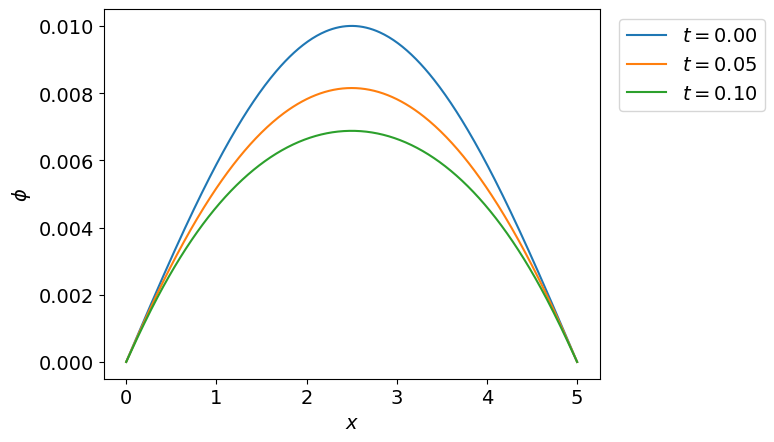
\includegraphics[width=\textwidth]{pictures/equilibrium_2_0.png}
    \vspace{-0.8cm}
    \caption{Случай среднего напряжения: возмущенное положение равновесия $\phi \equiv 0$, \linebreak устойчивое.}
    \label{picture_equilibrium_2_0}
    \vspace{0.5cm}

    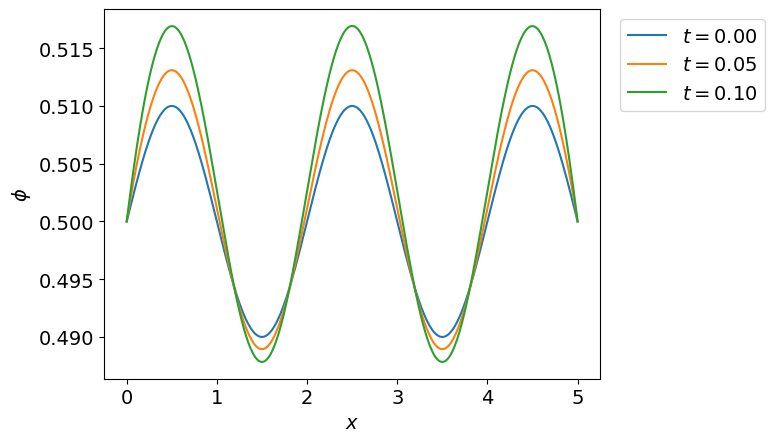
\includegraphics[width=\textwidth]{pictures/equilibrium_2_05.png}
    \vspace{-0.8cm}
    \caption{Случай среднего напряжения: возмущенное положение равновесия $\phi \equiv C_3 \hm \approx 0.5$, неустойчивое.}
    \label{picture_equilibrium_2_05}
    \vspace{0.5cm}
    
    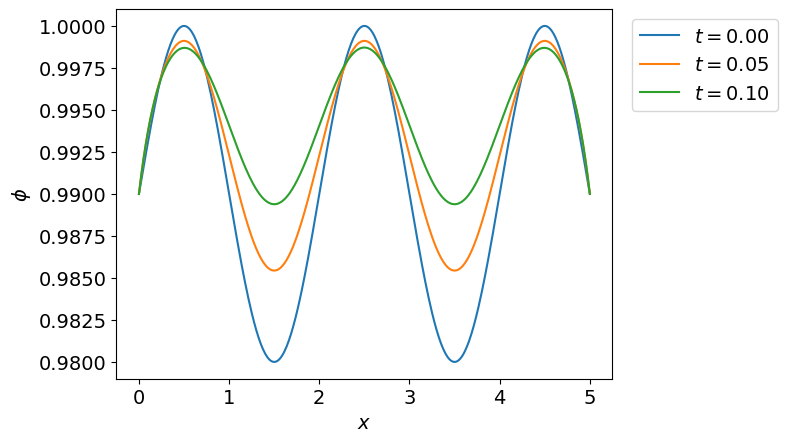
\includegraphics[width=\textwidth]{pictures/equilibrium_2_1.png}
    \vspace{-0.8cm}
    \caption{Случай среднего напряжения: возмущенное положение равновесия $\phi \equiv 1$, \linebreak устойчивое.}
    \label{picture_equilibrium_2_1}
\end{figure}

Наконец, рассмотрим $K_{\Phi, 3} = 4.8, \; \xi_3 > (1 + \delta)^2$ -- случай сильного напряжения. Система имеет два положения равновесия: $\phi \equiv 0$ устойчивое, $\phi \equiv 1$ неустойчивое. Поведение возмущенной среды изображено на рис. \ref{picture_equilibrium_3_0}, \ref{picture_equilibrium_3_1}, оно также соответствует теории.

\begin{figure}[!t]
    \centering
    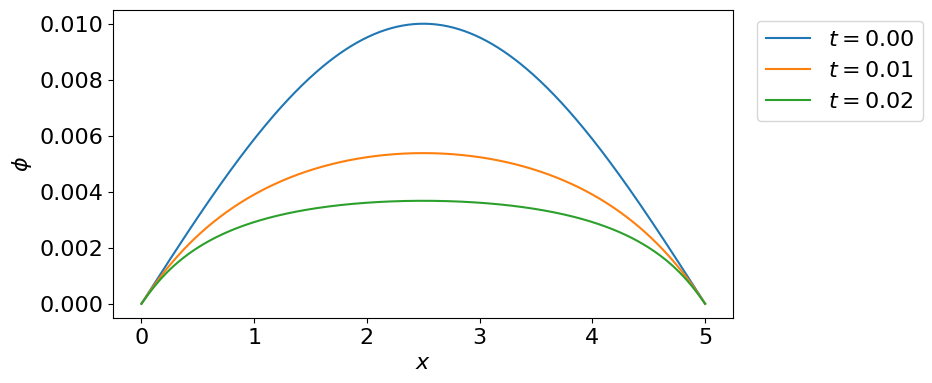
\includegraphics[width=\textwidth]{pictures/equilibrium_3_0.png}
    \vspace{-0.8cm}
    \caption{Случай сильного напряжения: возмущенное положение равновесия $\phi \equiv 0$, \linebreak устойчивое.}
    \label{picture_equilibrium_3_0}
    \vspace{0.5cm}
    
    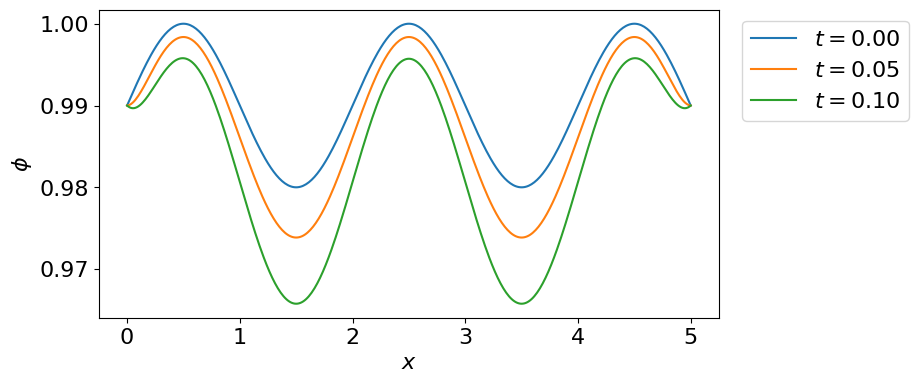
\includegraphics[width=\textwidth]{pictures/equilibrium_3_1.png}
    \vspace{-0.8cm}
    \caption{Случай сильного напряжения: возмущенное положение равновесия $\phi \equiv 1$, \linebreak неустойчивое.}
    \label{picture_equilibrium_3_1}
\end{figure}


\subsection{Вычислительный эксперимент: свободная энергия}

В рассматриваемой модели введена функция свободной энергии \eqref{equation_free_energy}, заданная интегралом плотности свободной энергии \eqref{equation_free_energy_density} по пространству. Плотность свободной энергии является суммой трех слагаемых -- обозначим их $\pi_1$, $\pi_2$ и $\pi_3$. В рассматриваемой одномерной задаче \eqref{equation_one_dim_simpler} выражения этих слагаемых принимают следующий вид. Плотность энергии электрического поля:

\begin{equation}
    \pi_1(x, t) = -\cfrac{1}{2} \epsilon[\phi] (\nabla \Phi, \nabla \Phi) = -\cfrac{K_\Phi^2}{2} \, \epsilon[\phi(x, t)] \text{.}
    \label{equation_free_energy_density_electrical}
\end{equation}
Плотность энергии, отнесенной к веществу внутри канала пробоя:
\begin{equation}
    \pi_2(x, t) = \Gamma \cfrac{1 - f[\phi(x, t)]}{l^2} \text{.}
    \label{equation_free_energy_density_inner}
\end{equation}
Плотность энергии, отнесенной к граничной зоне канала пробоя:
\begin{equation}
    \pi_3(x, t) = \cfrac{\Gamma}{4} (\nabla \phi, \nabla \phi) = \cfrac{\Gamma}{4} \left( \cfrac{\partial \phi}{\partial x}(x, t) \right)^2 \text{.}
    \label{equation_free_energy_density_border}
\end{equation}

Построим графики трех составляющих плотности свободной энергии системы с помощью программы и убедимся, что их поведение соответствует логике модели.

Зададим модели параметры \eqref{experiment_parameters}, \eqref{experiment_set} и краевые условия \eqref{experiment_borders}. Ранее мы уже проводили расчеты в этой конфигурации -- графики $\phi$ изображены на рис. \ref{picture_typical_solution}.

На основе уже реализованной схемы \eqref{scheme_transition}, \eqref{scheme_borders}  плотности энергии $\pi_1$ и $\pi_2$ \linebreak вычисляются тривиально; для расчета $\pi_3$ требуется вычислить разностную частную производную $\partial_h \phi_h / \partial_h x$. Используем для этого следующие формулы:
$$\cfrac{\partial_h \phi_h}{\partial_h x} \bigg|_a =
\begin{cases}
    (\phi_{a + 1} - \phi_{a - 1}) / (2h), \; \text{если} \; a = \overline{1, n - 1} \text{;} \\
    (\phi_1 - \phi_0) / h, \; \text{если} \; a = 0 \text{;} \\
    (\phi_n - \phi_{n - 1}) / h, \; \text{если} \; a = n \text{.}
\end{cases}$$

Полную свободную энергию системы найдем по формуле
$$\Pi_h = \sum\limits_{i = 0}^{n - 1} h \cfrac{\pi_{i + 1} + \pi_i}{2} = h \cfrac{\pi_0 + \pi_n}{2} + \sum\limits_{i = 1}^{n - 1} h \pi_i \text{.}$$

\begin{figure}[!tp]
    \centering
    \includegraphics[width=0.9\textwidth]{pictures/energy_density_electrical.png}
    \vspace{-0.3cm}
    \caption{Плотность энергии электрического поля.}
    \label{picture_energy_density_electrical}
    \vspace{0.5cm}
    
    \includegraphics[width=0.9\textwidth]{pictures/energy_density_inner.png}
    \vspace{-0.3cm}
    \caption{Плотность энергии, отнесенной к веществу внутри канала пробоя.}
    \label{picture_energy_density_inner}
    \vspace{0.5cm}
    
    \includegraphics[width=0.9\textwidth]{pictures/energy_density_border.png}
    \vspace{-0.3cm}
    \caption{Плотность энергии, отнесенной к граничной зоне канала пробоя.}
    \label{picture_energy_density_border}
\end{figure}

Результаты вычисления плотностей энергии $\pi_1$, $\pi_2$ и $\pi_3$ изображены на рис. \ref{picture_energy_density_electrical}, \ref{picture_energy_density_inner}, \ref{picture_energy_density_border} соответственно. Графики, относящиеся к одним и тем же моментам времени, имеют на них и на рис. \ref{picture_typical_solution} одинаковые цвета.

Сразу отметим, что отрицательные значения свободной энергии (и плотности энергии) не должны смущать: важны лишь их относительная величина и изменение.

На рис. \ref{picture_energy_density_electrical} и \ref{picture_energy_density_inner} видно, что по мере роста канала пробоя плотность энергии $\pi_1$ электрического поля падает (ввиду увеличения диэлектрической проницаемости $\epsilon$), плотность энергии $\pi_2$ вещества внутри канала, наоборот, растет. Обратим внимание, что, во-первых, $\pi_1$ имеет многократно больший диапазон значений, чем $\pi_2$, во-вторых, в момент $t \approx 0.55$ <<прорастания канала насквозь>> $\pi_1$ падает очень резко.

Посмотрим теперь на рис. \ref{picture_energy_density_border}. На графиках плотности энергии $\pi_3$ граничной зоны канала пробоя видны пары <<крутых>> симметричных пиков, которые постепенно, по мере роста канала в ширину, расходятся к краям отрезка $[0, 5]$. До момента $t \approx 0.55$ <<прорастания канала насквозь>> $\pi_3$ мала, так что ее графики были бы не видны на рисунке.

Результат вычисления полной свободной энергии $\Pi$ в зависимости от времени изображен на рис. \ref{picture_energy_total}. Для сравнения с предыдущими рисунками пунктирными линиями соответствующих цветов отмечены моменты времени. Интересно, что момента $t = 0.5$ энергия $\Pi$ убывает очень медленно; после, при $t \approx 0.55$, резко падает; затем падение замедляется, и после $t = 0.6$ убывание выравнивается, становясь близким к линейному; так продолжается практически до полного разрушения среды.

\begin{figure}
    \centering
    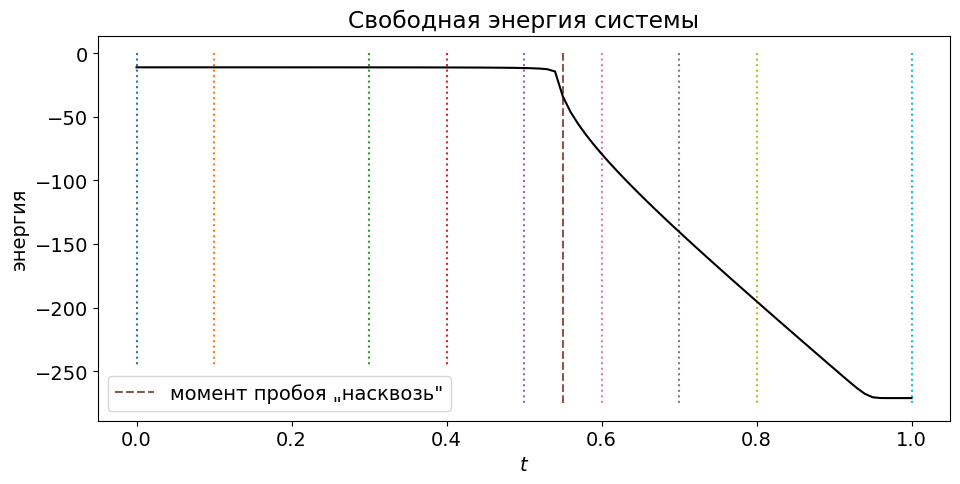
\includegraphics[width=\textwidth]{pictures/energy_total.png}
    \vspace{-0.5cm}
    \caption{Полная свободная энергия системы.}
    \label{picture_energy_total}
\end{figure}

Отметим, что вывод системы уравнений \eqref{equation_Phi}, \eqref{equation_phi} динамики системы из выражения~\eqref{equation_free_energy} для свободной энергии означает, что система в ходе эволюции стремится в положение с как можно меньшей свободной энергией. Поэтому для адекватного моделирования системы крайне важно, чтобы полная свободная энергия $\Pi$ не возрастала. Мы не дали этому теоретического обоснования для используемой разностной схемы, однако проверили на опыте. Другими словами, это означает, что при используемом виде краевых условий и параметрах расчета предложенная схема является градиентно-устойчивой.

Итак, экспериментально подтверждено, что поведение полной свободной энергии и трех составляющих плотности свободной энергии вполне подчиняется логике исследуемой модели.


\section{Обобщение модели}
\label{section_model_fixing}

\subsection{Суть проблемы}
\label{subsection_matter_of_problem}

Как говорилось ранее, исследуемая модель канала электрического пробоя, предложенная в работе \cite{pitike_dielectric_breakdown}, создана на основе подобных моделей из теории трещин. Учитывая это, ознакомимся с анализом модели в следующем характеристическом случае.

Рассмотрим систему уравнений \eqref{equation_Phi}, \eqref{equation_phi} с упрощающими краевыми условиями, описанными в подразделе \ref{subsection_one_dimensional_problem}. Как было показано, система сведется к единственному нетривиальному уравнению \eqref{equation_one_dim_simpler} одной пространственной переменной $x$ и времени $t$ на фазовое поле $\phi$. Пусть $K_\Phi = 0$ (электрическое напряжение нулевое); будем искать стационарное решение следующей краевой задачи: $\phi(0) = 0, \; \phi(x) \to 1$ при $x \to +\infty$.

Уравнение \eqref{equation_one_dim_simpler} принимает следующий вид:
$$f'(\phi) = - \cfrac{l^2}{2} \cfrac{\partial^2 \phi}{\partial x^2} \text{.}$$
Домножим обе части уравнения на $\phi'_x$. Учитывая, что $f'_\phi \phi'_x = f'_x$ и $2 \phi'_x \phi''_{xx} = [(\phi'_x)^2]'_x$, проинтегрируем и, с учетом $\phi \to 1, \; \phi'_x \to 0$ при $x \to \infty$, получим:
\begin{equation}
    \cfrac{\partial \phi}{\partial x} = \cfrac{2}{l} \sqrt{1 - f(\phi)} \text{.}
    \label{equation_stationary_rectangular}
\end{equation}
Итак, мы перешли к обыкновенной задаче Коши с уравнением \eqref{equation_stationary_rectangular} и условием $\phi(0) = 0$.

Рассмотренный случай системы имеет следующий смысл: найдено распределение фазового поля в полупространстве сбоку от проводящей пластины (состоящей из полностью разрушенного вещества). Этот случай был ранее назван характеристическим, так как показывает влияние на систему параметра $l$: видно, что $l$ в уравнении~\eqref{equation_stationary_rectangular} есть коэффициент <<растяжения>> решения вдоль оси $x$. Можно показать \cite{zipunova_higher_codimension}, что при $x > l$ решение рассмотренной задачи Коши $\phi \approx 1$. Другими словами, решение есть распределение фазового поля, локализованное на отрезке $[0, l]$.

Подобный анализ вполне подходит для задачи из теории трещин (вместо проводящей пластины была бы плоская трещина). Однако характерный канал пробоя -- объект не двумерный, а одномерный. Проверим, можно ли провести аналогичное рассуждение не для пластины, а для тонкого прямого проводника.

Рассмотрим систему уравнений \eqref{equation_Phi}, \eqref{equation_phi} в области $\Omega = \mathbb{R}_x \times \mathbb{R}_y \times I_z$, где $I$ -- некоторый отрезок, при условии, что $\Phi \equiv 0$ (электрическое напряжение нулевое). Уравнение~\eqref{equation_Phi} выполняется тождественно, осталось единственное нетривиальное уравнение \eqref{equation_phi} на $\phi$. Будем искать стационарное решение следующей краевой задачи: $\phi|_{x, y = 0} = 0, \; \phi \to 1$ при $r = \sqrt{x^2 + y^2} \to +\infty$.

Удобно перейти в цилиндрическую систему координат: $x, y, z \longmapsto r, \theta, z$. Граничные условия однородны по $\theta$ и $z$, поэтому естественно искать решение, зависящее только от $r$. Так как $\phi(\mathbf{x}) = \phi(r)$, выражение для лапласиана $\phi$ в цилиндрических координатах принимает следующий вид:
$$\triangle \phi = \cfrac{1}{r} \cfrac{\partial}{\partial r} \left( r \cfrac{\partial \phi}{\partial r} \right) = \cfrac{1}{r} \cfrac{\partial \phi}{\partial r} + \cfrac{\partial ^2 \phi}{\partial r^2} \text{.}$$
С учетом этого уравнение \eqref{equation_phi} преобразуется в
\begin{equation}
    \cfrac{2}{l^2} f'(\phi) + \cfrac{1}{r} \cfrac{\partial \phi}{\partial r} + \cfrac{\partial ^2 \phi}{\partial r^2} = 0 \text{.}
    \label{equation_stationary_cylindrical}
\end{equation}

Подобное рассуждение проделано в работе \cite{zipunova_higher_codimension}; за ним следует анализ уравнения~\eqref{equation_stationary_cylindrical}. На основании теоретических результатов из работы \cite{cirstea_elliptic_equations} заключается, что поставленная краевая задача некорректна и решения не имеет. Даже на уровне интуиции постановка задачи выглядит необычно: условие $\phi|_{x, y = 0} = 0$ задано не на двумерной, а на одномерной <<внутренней>> границе области $\Omega$.

Возникает желание формально изменить модель так, чтобы описанная краевая задача имела решение. При моделировании канал пробоя невозможно явно представить сегментом линии, за исключением тривиальных случаев, -- однако естественно считать его <<нитевидной>> областью соответствующей формы, радиус которой может стремиться к нулю. Распределение фазового поля вблизи канала пробоя в таком случае должно приближаться к решению рассмотренной краевой задачи.

\pagebreak


\subsection{Предложенное обобщение}

В ответ на описанную в предыдущем подразделе проблему в работе \cite{zipunova_higher_codimension}, на основании теоретических результатов работ \cite{sobolev_functional_analysis}, \cite{oleynik_biharmonic_equations}, \cite{sternin_elliptic_equations}, \cite{lewis_quasi_linear}, предлагается следующая обобщенная модель, для которой постановка условий на границах размерности 1 (соответственно, коразмерности 2) является математически корректной:
\begin{equation}
    \Pi = \int \limits_\Omega \pi d \mathbf{x} \text{,}
    \label{equation_free_energy_corrected}
\end{equation}
\begin{equation}
    \pi = -\cfrac{1}{2} \epsilon[\phi] (\nabla \Phi, \nabla \Phi) + \Gamma \cfrac{1 - f(\phi)}{l^2} + \cfrac{\Gamma}{4} (\nabla \phi, \nabla \phi) + \alpha \cfrac{\Gamma l^2}{8} (\triangle \phi)^2 + \beta \cfrac{1}{p} \Gamma l^{p - 2} \| \, \nabla \phi \, \|_2^p \text{;}
    \label{equation_free_energy_density_corrected}
\end{equation}
\begin{numcases}{}
    \Div(\epsilon[\phi] \nabla \Phi) = 0 \text{;} \label{equation_Phi_corrected} \\
    \cfrac{1}{m} \cfrac{\partial \phi}{\partial t} = \cfrac{1}{2} \epsilon'(\phi) (\nabla \Phi, \nabla \Phi) + \cfrac{\Gamma}{l^2} f'(\phi) + \cfrac{1}{2} \Gamma \triangle \phi - \alpha \cfrac{\Gamma l^2}{4} \triangle^2 \phi + \beta \Gamma l^{p - 2} \Div (\| \, \nabla \phi \, \|_2^{p - 2} \nabla \phi) \text{.}
    \label{equation_phi_corrected}
\end{numcases}
Здесь $\alpha, \beta \geqslant 0$ -- некоторые константы, $p$ -- четное натуральное число, не меньшее~4. Дифференциальный оператор $\Div (\| \, \nabla \phi \, \|_2^{p - 2} \nabla \phi)$ принято называть \emph{$p$-лапласианом}, \linebreak $\triangle^2 \phi = \triangle(\triangle \phi)$ -- \emph{билапласианом}. В дальнейшем для простоты будем считать $p = 4$.


\subsection{О методе конечных объемов}

Нашей целью будет численно исследовать систему уравнений \eqref{equation_Phi_corrected}, \eqref{equation_phi_corrected} в трех характеристических случаях, подобных описанному в подразделе \ref{subsection_matter_of_problem}.

Итак, мы ищем стационарное решение задачи \eqref{equation_Phi_corrected}, \eqref{equation_phi_corrected} с $\Phi \equiv 0$ для трех различных граничных условий:
\begin{enumerate}
    \item $\Omega = [0, +\infty)_x \times I_y \times I_z, \; \phi|_{x = 0} = 0, \; \phi \to 1$ при $x \to +\infty$ -- плоский случай;
    \item $\Omega = \mathbb{R}_x \times \mathbb{R}_y \times I_z, \; \phi|_{x, y = 0} = 0, \; \phi \to 1$ при $r = \sqrt{x^2 + y^2} \to +\infty$ -- цилиндрический случай;
    \item $\Omega = \mathbb{R}_x \times \mathbb{R}_y \times \mathbb{R}_z, \; \phi|_{x, y, z = 0} = 0, \; \phi \to 1$ при $r = \sqrt{x^2 + y^2 + z^2} \to +\infty$ -- сферический случай.
\end{enumerate}
Подробно случаи 1 и 2 были описаны в подразделе \ref{subsection_matter_of_problem}. Случай 3 закономерно продолжает ряд: в нем граничное условие задано в точке -- объекте коразмерности 3.

Стационарное решение соответствует минимуму свободной энергии $\Pi$. Уравнения динамики системы выведены таковыми, что система стремится к минимуму энергии $\Pi$ в ходе эволюции. Поэтому будем проводить расчет на достаточно долгое время, тогда установившееся положение равновесия и будет искомым стационарным решением $\phi$.

В случаях 2 и 3 естественно перейти в цилиндрические и сферические координаты соответственно и считать решение $\phi$ зависящим только от радиуса $r$. В случае 1 для единообразия пространственную переменную также назовем $r$. Итак, $\phi(\mathbf{x}) = \phi(r)$.

Для численного решения задачи воспользуемся методом конечных объемов. \linebreak Классический метод конечных разностей, встречая ряд проблем, подходит плохо. К примеру, в уравнениях разностной схемы могут возникать ситуации деления на 0 в узле $r = 0$ в цилиндрическом и сферическом случае (см. формулу \eqref{equation_stationary_cylindrical}).

При моделировании мы ограничим область $\Omega$ некоторым конечным размером -- граничные условия превращаются в $\phi(0) = 0, \; \phi(R) = 1, \; R > 0$ -- внешний радиус $\Omega$, такой что $R / l \gg 1$.

Разобьем область $\Omega$ на $n + 1$ ячейку (прямоугольную либо в форме цилиндрического или сферического слоя), обозначим их $\Omega_0, ..., \Omega_n$. Пусть границы ячеек имеют радиусы $0 = r_{-1/2}, r_{1/2}, ..., r_{n + 1/2} = R$.

Обозначим $V(r)$ объем прямоугольника, цилиндра или сферы (в зависимости от случая), который заполняет область $\Omega$ от радиуса $0$ до $r$. Пусть $S(r)$ -- площадь внешней (разделяющей область $\Omega$) поверхности подобного прямоугольника, цилиндра или сферы. Тогда объем ячейки $\Omega_i$ равен $dV_i = V(r_{i + 1/2}) - V(r_{i - 1/2})$, площадь внутренней и внешней границ -- $S(r_{i - 1/2})$ и $S(r_{i + 1/2})$ соответственно.

\begin{enumerate}[label=\arabic*.]
    \item Плоский случай. $V(r) = r \cdot |I_y| \cdot |I_z|, \; S(r) = |I_y| \cdot |I_z|$. Сократив, можно считать $V(r) = r, \; S(r) = 1$.
    \item Цилиндрический случай. $V(r) = \pi r^2 \cdot |I_z|, \; S(r) = 2 \pi r \cdot |I_z|$. Сократив, можно считать $V(r) = r^2, \; S(r) = 2r$.
    \item Сферический случай. $V(r) = (4/3) \pi r^3, \; S(r) = 4 \pi r^2$. Домножив оба выражения на $3/(4\pi)$, можно считать $V(r) = r^3, \; S(r) = 3 r^2$.
\end{enumerate}

Итак, было показано, что можно считать $V(r) = r^{k + 1}, \; S(r) = (k + 1)r^k$, где $k = 0$ для плоского случая, $k = 1$ для цилиндрического, $k = 2$ для сферического.

Проведем преобразование решаемого уравнения \eqref{equation_phi_corrected}, обычное для метода конечных объемов. Учтем, что $\Phi \equiv 0$. Уравнение представляется в следующей форме:
\begin{equation}
    \cfrac{1}{m} \cfrac{\partial \phi}{\partial t} = \cfrac{\Gamma}{l^2} f'(\phi) + \Gamma \Div \overline{\rho} \text{,}
    \label{equation_phi_for_integration}
\end{equation}
где
$$\overline{\rho} = \cfrac{1}{2} \nabla \phi - \alpha \cfrac{l^2}{4} \nabla (\triangle \phi) + \beta l^2 \| \, \nabla \phi \, \|_2^2 \nabla \phi \text{.}$$
Проинтегрируем уравнение \eqref{equation_phi_for_integration} вначале по некоторому промежутку времени [$t_j, t_{j + 1}]$, затем по ячейке $\Omega_i$. Преобразуем левую часть:
$$\int\limits_{\Omega_i} \int\limits_{t_j}^{t_{j + 1}} \cfrac{1}{m} \cfrac{\partial \phi}{\partial t} dt d \mathbf{x} = \cfrac{1}{m} \int\limits_{\Omega_i} [\phi(\mathbf{x}, t_{j + 1}) - \phi(\mathbf{x}, t_j)] d \mathbf{x} = \cfrac{dV_i}{m} [\widetilde{\phi}_i(t_{j + 1}) - \widetilde{\phi}_i(t_j)] \text{,}$$
где $\widetilde{\phi}_i$ -- это интегральное среднее функции $\phi$ по ячейке $\Omega_i$. Преобразуем правую часть, предварительно поменяв порядок интегрирования:
$$\int\limits_{t_j}^{t_{j + 1}} \int\limits_{\Omega_i} \left( \cfrac{\Gamma}{l^2} f'(\phi) + \Gamma \Div \overline{\rho} \right) d \mathbf{x} dt = \int\limits_{t_j}^{t_{j + 1}} \left( \cfrac{\Gamma}{l^2} \int\limits_{\Omega_i} f'(\phi) d \mathbf{x} + \Gamma \int\limits_{\partial \Omega_i} (\overline{\rho}, \overline{n}) dS \right) dt \text{.}$$
К интегралу слагаемого $\Gamma \Div \overline{\rho}$ была применена формула Гаусса--Остроградского. Функция $\phi$ зависит только от $r$, следовательно, вектор $\overline{\rho}$ всегда параллелен оси $r$. Граница ячейки $\partial \Omega_i$ складывается из внешней (где вектор нормали $\overline{n}$ и ось $r$ сонаправлены) и внутренней (где $\overline{n}$ и ось $r$ противоположно направлены). Обозначим $F_{i \pm 1/2}(t)$ поток в положительном направлении оси $r$ через соответствующую границу с радиусом $r_{i \pm 1/2}$:
$$F_{i \pm 1/2}(t) = \int\limits_{r = r_{i \pm 1/2}} (\overline{\rho}, \overline{n}) dS = \int\limits_{r = r_{i \pm 1/2}} \overline{\rho}_r dS = \overline{\rho}_r S(r_{i \pm 1/2}) = \rho_{i \pm 1/2}(t) \cdot S(r_{i \pm 1/2}) \text{,}$$
$$\int\limits_{\partial \Omega_i} (\overline{\rho}, \overline{n}) dS = F_{i + 1/2} - F_{i - 1/2} = \rho_{i + 1/2} S(r_{i + 1/2}) - \rho_{i - 1/2} S(r_{i - 1/2}) \text{.}$$
Здесь $\overline{\rho}_r$ обозначена $r$-координата вектора $\overline{\rho}$ (она же единственная ненулевая). Величину $\rho_{i \pm 1/2}(t) = \overline{\rho}_r(r_{i \pm 1/2}, t)$ будем называть плотностью потока через соответствующую границу. Таким образом, выведено следующее интегральное соотношение:
\begin{equation}
    \cfrac{dV_i}{m} [\widetilde{\phi}_i(t_{j + 1}) - \widetilde{\phi}_i(t_j)] = \int\limits_{t_j}^{t_{j + 1}} \left( \cfrac{\Gamma}{l^2} \int\limits_{\Omega_i} f'(\phi) d \mathbf{x} + \Gamma \left[ \rho_{i + 1/2} S(r_{i + 1/2}) - \rho_{i - 1/2} S(r_{i - 1/2}) \right] \right) dt \text{.}
    \label{equation_finite_volume_integral}
\end{equation}

Первое слагаемое в подынтегральном выражении в правой части равенства \eqref{equation_finite_volume_integral} приблизим выражением $(\Gamma/l^2) \cdot dV_i \cdot f'[\widetilde{\phi}_i(t_j)]$. При построении разностной схемы от интеграла по $[t_j, t_{j + 1}]$ перейдем к умножению на $(t_{j + 1} - t_j)$ значения подынтегрального выражения в точке $t_j$.

Выясним, как вычислить плотность потока $\rho_{i \pm 1/2}$ во втором слагаемом. Если некоторая функция $\psi(\mathbf{x}) = \psi(r)$, то
$$(\nabla \psi)_r = \cfrac{\partial \psi}{\partial r} \text{,}$$
где $\nabla \psi$ также зависит только от $r$. Таким образом:
\begin{equation}
    \rho = \cfrac{1}{2} \cfrac{\partial \phi}{\partial r} - \alpha \cfrac{l^2}{4} \cfrac{\partial}{\partial r} (\triangle \phi) + \beta l^2 \left( \cfrac{\partial \phi}{\partial r} \right)^3 \text{.}
    \label{equation_finite_volumes_density}
\end{equation}

Традиционно в методе конечных объемов принимается, что локальное восполнение решения в ячейке -- постоянная функция. В силу того, что рассматриваемая задача требует постановки граничных условий при $r = 0$, а решение задачи вблизи этой точки может иметь большие производные, обобщим традиционный подход. А именно, будем считать, что в окрестности нуля решение представляется в виде линейной комбинации двух специально выбранных базисных функций, а его производные, соответственно, приближаются линейной комбинацией производных базисных функций с теми же коэффициентами. Опишем в общем виде поиск коэффициентов разложения.

Построим приближение для некоторой функции $\psi(r)$ в соседних ячейках $\Omega_i$ и $\Omega_{i + 1}$ по известным интегральным средним $\widetilde{\psi}_i$ и $\widetilde{\psi}_{i + 1}$ в этих ячейках. Пусть
$$g(r) = a \cdot g^{(a)}(r) + b \cdot g^{(b)} (r)$$
есть функция с двумя числовыми параметрами $a$ и $b$, $g^{(a)}$ и $g^{(b)}$ -- базисные функции, используемые для локального представления $\psi$. Найдем такие $a$ и $b$, что интегральные средние $g(r)$ по ячейкам $\Omega_i$ и $\Omega_{i + 1}$ были бы равны $\widetilde{\psi}_i$ и $\widetilde{\psi}_{i + 1}$ соответственно. Это эквивалентно системе уравнений
\begin{numcases}{}
    \int\limits_{r_{i - 1/2}}^{r_{i + 1/2}} [\widetilde{\psi}_i - g(r)] S(r) dr = 0 \text{;}
    \label{equation_interpolation_first} \\
    \int\limits_{r_{i + 1/2}}^{r_{i + 3/2}} [\widetilde{\psi}_{i + 1} - g(r)] S(r) dr = 0 \text{.}
    \label{equation_interpolation_second}
\end{numcases}
Пусть
$$\int\limits_{r_{i - 1/2}}^{r_{i + 1/2}} g^{(a)}(r) S(r) dr = I_i^{(a)}; \qquad \int\limits_{r_{i - 1/2}}^{r_{i + 1/2}} g^{(b)}(r) S(r) dr = I_i^{(b)} \text{.}$$
Считаем, что интегралы $I_i^{(a)}$ и $I_i^{(b)}$ найдены аналитически. Тогда система \eqref{equation_interpolation_first}, \eqref{equation_interpolation_second} эквивалентна системе
$$\begin{cases}
    a I_i^{(a)} + b I_i^{(b)} = (r_{i + 1/2}^{k + 1} - r_{i - 1/2}^{k + 1}) \widetilde{\psi}_i \text{;} \\
    a I_{i + 1}^{(a)} + b I_{i + 1}^{(b)} = (r_{i + 3/2}^{k + 1} - r_{i + 1/2}^{k + 1}) \widetilde{\psi}_{i + 1} \text{.}
\end{cases}$$
Это система двух линейных уравнений с двумя неизвестными -- решим методом Крамера. Получим:
$$\varDelta = I_i^{(a)} I_{i + 1}^{(b)} - I_i^{(b)} I_{i + 1}^{(a)} \text{;}$$
\begin{equation}
    a = \cfrac{(r_{i + 1/2}^{k + 1} - r_{i - 1/2}^{k + 1}) I_{i + 1}^{(b)}}{\varDelta} \cdot \widetilde{\psi}_i + \cfrac{-(r_{i + 3/2}^{k + 1} - r_{i + 1/2}^{k + 1}) I_i^{(b)}}{\varDelta} \cdot \widetilde{\psi}_{i + 1} \text{;}
    \label{equation_interpolation_a}
\end{equation}
\begin{equation}
    b = \cfrac{-(r_{i + 1/2}^{k + 1} - r_{i - 1/2}^{k + 1}) I_{i + 1}^{(a)}}{\varDelta} \cdot \widetilde{\psi}_i + \cfrac{(r_{i + 3/2}^{k + 1} - r_{i + 1/2}^{k + 1}) I_i^{(a)}}{\varDelta} \cdot \widetilde{\psi}_{i + 1} \text{.}
    \label{equation_interpolation_b}
\end{equation}
Теперь можно легко находить $a$ и $b$ при различных значениях $\widetilde{\psi}_i, \; \widetilde{\psi}_{i + 1}$, если вычислить заранее и сохранить четыре коэффициента, стоящие в формулах \eqref{equation_interpolation_a}, \eqref{equation_interpolation_b}. 

Приблизим $\partial \psi / \partial r$ на границе с радиусом $r_{i + 1/2}$ (между ячейками $\Omega_i$ и $\Omega_{i + 1}$) с помощью функции $g(r)$ с известными числовыми параметрами:
$$\left[ \cfrac{\partial \psi}{\partial r} \right]_{i + 1/2} = g'(r_{i + 1/2}) = a \cdot (g^{(a)})'(r_{i + 1/2}) + b \cdot (g^{(b)})'(r_{i + 1/2}) \text{.}$$
Производные $(g^{(a)})'$ и $(g^{(b)})'$ считаем найденными аналитически.

Отыщем приближение производной $\partial \phi / \partial r$ на границах с радиусами $r_{3/2}, ...$, $r_{n - 1/2}$ (то есть на всех, кроме первых двух внутренних и крайней внешней). Используем описанный выше метод с $\widetilde{\psi} = \widetilde{\phi}$ и базисными функциями $g^{(a)}(r) = r, \; g^{(b)}(r) = 1$. $g' \equiv a$, вывести формулы для $I^{(a)}$, $I^{(b)}$ также не составляет труда. Таким образом, происходит приближение функции $\phi$ на парах соседних ячеек линейной функцией.

Задание граничных условий, в том числе приближение $\partial \phi / \partial r$ на крайних границах $\Omega$, будет подробно описано в следующем разделе.

Без ответа остался только вопрос вычисления $\triangle \phi$ и его производной по $r$. Оно требуется лишь в случае ненулевой константы $\alpha$ (см. уравнение \eqref{equation_phi_corrected}). Проведя рассуждение, аналогичное проделанному для вывода соотношения \eqref{equation_finite_volume_integral}, но без интегрирования по времени, получим следующее выражение для интегрального среднего лапласиана $\phi$ по ячейке:
\begin{equation}
    dV_i \cdot \widetilde{\triangle \phi}_i = \cfrac{\partial \phi}{\partial r} \bigg|_{r = r_{i + 1/2}} S(r_{i + 1/2}) - \cfrac{\partial \phi}{\partial r} \bigg|_{r = r_{i - 1/2}} S(r_{i - 1/2}) \text{.}
    \label{equation_finite_volume_laplasian}
\end{equation}

По средним $\widetilde{\triangle \phi}$ вычислим приближение $\partial (\triangle \phi) / \partial r$ на границах ячеек с радиусами $r_{1/2}, ..., r_{n - 1/2}$ (то есть на всех, кроме крайних внутренней и внешней) тем же способом, который ранее использовался для $\partial \phi / \partial r$, с $\widetilde{\psi} = \widetilde{\triangle \phi}, \; g^{(a)}(r) \hm = r, \; g^{(b)}(r) = 1$.


\subsection{Задание граничных условий}

Граничные условия, подробно описанные в предыдущем разделе, имеют следующий вид: $\phi(0) = 0, \; \phi(R) = 1, \; R > 0$, где $R$ такое, что $R / l \gg 1$. Если коэффициент $\alpha$ в уравнении \eqref{equation_phi_corrected} при слагаемом с билапласианом ненулевой, то этих граничных условий недостаточно в силу повышения порядка уравнения -- необходимо добавить условия на производные. По логике задачи их следует сделать таковыми:
$$\cfrac{\partial \phi}{\partial r} \bigg|_{r = 0} = 0, \qquad \cfrac{\partial \phi}{\partial r} \bigg|_{r = 1} = 0 \text{.}$$

Граничные условия в точке $r = R$ в разностной схеме задаются легко: $\widetilde{\phi}_n \hm \equiv 1, \; \widetilde{\triangle \phi}_n \equiv 0$. Этого оказывается достаточно ввиду того, что функция $\phi$ вблизи точки $R$ меняется очень слабо.

С граничными условиями в точке $r = 0$ дела обстоят намного сложнее. Для начала, функции перехода в цилиндрическую и сферическую систему координат имеют в этой точке особенность. К тому же ожидается, что $\phi$ в окрестности точки $r = 0$ довольно быстро растет. Более того, как выяснится позже, в цилиндрическом и сферическом случае в точке $0$ имеют особенность производные функций $\phi$ и $\triangle \phi$.

Зададим граничные условия в точке $0$ следующим образом. Выберем для приближения $\phi$ в ячейках $\Omega_0$ и $\Omega_1$ такие базисные функции $g^{(a)}$ и $g^{(b)}$, что каждая из них удовлетворяет граничным условиям при $r = 0$ и, при необходимости, одна из них имеет в точке $0$ предположительно тот же вид особенности, что решение $\phi$. С помощью функции $g(r)$ с известными параметрами получим искомые приближения:
$$\left[ \cfrac{\partial \phi}{\partial r} \right]_{-1/2} = g'(0); \qquad \left[ \cfrac{\partial \phi}{\partial r} \right]_{1/2} = g'(r_{1/2}) \text{;}$$
$$\left[ \cfrac{\partial (\triangle \phi)}{\partial r} \right]_{-1/2} = \cfrac{\partial}{\partial r} \left[ r^k \cfrac{\partial}{\partial r} \left(\cfrac{1}{r^k} \cfrac{\partial g}{\partial r} \right) \right] \Bigg|_{r = 0} \text{.}$$
В последнем выражении используется общий вид формулы для лапласиана функции, зависящей только от $r$, в прямоугольных, цилиндрических и сферических координатах:
\begin{equation}
    \triangle g = \cfrac{1}{r^k} \cfrac{\partial}{\partial r} \left( r^k \cfrac{\partial g}{\partial r} \right) \text{.}
    \label{equation_laplasian_common}
\end{equation}

Определимся с выбором базисных функций для приближения $\phi$ в первых двух ячейках в зависимости от случая задачи и значений параметров $\alpha$ и $\beta$.

Рассмотрим плоский случай. Здесь у производной $\phi$ (и $\triangle \phi$, входящей в формулы, только если $\alpha \neq 0$) в точке $0$ не ожидается особенностей. Обоснуем это так: $S(0) = 1 \hm \neq 0$, поэтому для ненулевого потока $F_{-1/2}$ через крайнюю внутреннюю границу нужна ненулевая конечная плотность потока $\rho_{-1/2}$. При $\alpha = 0$ граничное условие $\phi(0) = 0$ -- возьмем $g^{(a)} = r^2, \; g^{(b)} = r$. При $\alpha \neq 0$ добавляется граничное условие $\partial \phi / \partial r |_{r = 0} = 0$ -- используем $g^{(a)} = r^3, \; g^{(b)} = r^2$.

Теперь рассмотрим цилиндрический случай. Имеем $S(0) = 0$, поэтому, казалось бы, поток $F_{-1/2}$ всегда нулевой. Однако если допустить у $\rho$ особенность вида $1/r$, то получается $\rho(r) S(r) \to 2$ при $r \to +0$ -- конечный ненулевой поток! Если $\rho$ по модулю растет асимптотически медленнее, то поток будет нулевым, если быстрее, то бесконечным (что не имеет смысла).

Пусть $\alpha = \beta = 0$. Тогда в выражении \eqref{equation_finite_volumes_density} для плотности потока встречается лишь $\partial \phi / \partial r$ в первой степени. Значит, мы ищем $g^{(a)}$, такую что $(g^{(a)})' = C_0/r$. Проинтегрировав, получим $g^{(a)} = C_0 \ln r + C_1$. $g^{(a)} \to \infty$ при $r \to +0$, то есть граничное условие $g^{(a)}(0) = 0$ выполнить невозможно. Это косвенно подтверждает вывод из работы \cite{zipunova_higher_codimension}, что в этом случае решения дифференциальной задачи не существует.

Пусть $\alpha = 0, \; \beta \neq 0$. В выражение \eqref{equation_finite_volumes_density} для плотности потока входит $\partial \phi / \partial r$ в первой и третьей степени. Следовательно, мы ищем $g^{(a)}$, такую что $(g^{(a)})' = C_0 r^{-1/3}$. Ее первая степень даст нулевой вклад в поток, а третья -- конечный ненулевой. Проинтегрировав, получим $g^{(a)} = C_0 \cdot (3/2) \cdot r^{2/3} + C_1$. С учетом граничного условия выберем $g^{(a)} = r^{2/3}$. Вторую базисную функцию возьмем без особенности в точке $0$, например, $g^{(b)} = r$.

Пусть $\alpha \neq 0, \; \beta$ произвольное. Тогда в выражение \eqref{equation_finite_volumes_density} для плотности потока входит $\partial (\triangle \phi) / \partial r$. Встречается там и $\partial \phi / \partial r$, но она, согласно граничному условию, равна~$0$ при $r = 0$. Отыщем такую базисную функцию $g^{(a)}$, что $\partial (\triangle g^{(a)}) / \partial r = C_0 / r$. Учтем, что лапласиан функции $g^{(a)}$, зависящей только от $r$, в цилиндрических координатах вычисляется по формуле \eqref{equation_laplasian_common} с $k = 1$. Трижды проинтегрировав уравнение на производную лапласиана, получим $g^{(a)} = (C_0/4) r^2 (\ln r - 1) + C_1 r^2 / 4 + C_2 \ln r + C_3$. Требуется $g^{(a)}(0) = 0$, следовательно, $C_2 = C_3 = 0$. Особенность содержит первое слагаемое, поэтому выберем $g^{(a)} = r^2 (\ln r - 1)$. $g^{(a)}$ удовлетворяет граничному условию на производную $\partial g^{(a)} / \partial r|_{r = 0} = 0$. Второй базисной функцией сделаем $g^{(b)} = r^2$.

Наконец, рассмотрим сферический случай. Аналогично цилиндрическому случаю будем подбирать базисную функцию так, чтобы поток $F_{-1/2}$ был конечным. Для этого $\rho$ должна иметь особенность вида $1/r^2$, так как тогда $\rho(r) S(r) \to 3$ при $r \to 0$.

Пусть $\alpha = \beta = 0$. Аналогично рассмотренному ранее случаю ищем $g^{(a)}$, такую что $(g^{(a)})' = C_0 / r^2$. Проинтегрировав, получим $g^{(a)} = -C_0 / r + C_1$. $g^{(a)} \to \infty$ при $r \to +0$, то есть граничное условие $g^{(a)}(0) = 0$ выполнить невозможно.

Пусть $\alpha = 0, \; \beta \neq 0$. Аналогично рассмотренному ранее случаю ищем $g^{(a)}$, такую что $(g^{(a)})' = C_0 / r^{-2/3}$. Проинтегрировав, получим $g^{(a)} = C_0 \cdot 3 \cdot r^{1/3} + C_1$. С учетом граничного условия выберем $g^{(a)} = r^{1/3}, \; g^{(b)} = r$.

Пусть $\alpha \neq 0, \; \beta$ произвольное. Аналогично рассмотренному ранее случаю ищем $g^{(a)}$, такую что $\partial (\triangle g^{(a)}) / \partial r = C_0 / r^2$. Лапласиан функции $g^{(a)}$, зависящей только от $r$, в сферических координатах вычисляется по формуле \eqref{equation_laplasian_common} с $k = 2$. Дважды проинтегрировав уравнение на производную лапласиана, получим $(g^{(a)})' = -C_0 / 2 + C_1 r / 3 + C_2 / r^2$. $C_0 \neq 0$, так как иначе у функции пропадет особенность. Получается, что $(g^{(a)})'(0) \neq 0$ -- невозможно удовлетворить граничному условию на производную!

Примечательно, что выбранный подход не удалось применить в сферическом случае не только при $\alpha = \beta = 0$, но и при $\alpha \neq 0$. Выдвинем гипотезу, что в обеих этих конфигурациях исследуемая дифференциальная задача поставлена некорректно и не имеет решения.


\subsection{Разностная схема}

Везде в двух предыдущих подразделах допускалось, что радиусы границ ячеек $0 = r_{-1/2}, r_{1/2}, ..., r_{n - 1/2}, r_{n + 1/2} = R$ могут быть произвольной возрастающей последовательностью чисел. В дальнейшем, на практике, мы сделаем их структуру регулярной с шагом $h$: $r_{i - 1/2} = ih$.

При моделировании система будет проходить моменты времени $t_j = j \tau$, где $\tau$ -- фиксированный шаг по времени. Функцию времени с аргументом $t_j$ будем обозначать верхним индексом $j$.

В качестве начального условия задаются $\{ \widetilde{\phi}_i^0 \}_{i = 0}^n$.

Как было принято ранее, $k = 0$ в плоском случае, $k = 1$ в цилиндрическом, $k = 2$ в сферическом.

Подводя итог рассуждениям, проделанным в двух предыдущих подразделах, выпишем построенную методом конечных объемов разностную схему.

\begin{equation}
    \begin{gathered}
        \cfrac{1}{m} (\widetilde{\phi}_i^{j + 1} - \widetilde{\phi}_i^j) = \tau \cfrac{\Gamma}{l^2} f'(\widetilde{\phi}_i^j) + \cfrac{\tau}{dV_i} \Gamma (\rho_{i + 1/2}^j S_{i + 1/2} - \rho_{i - 1/2}^j S_{i - 1/2}) \; \text{при} \; i = \overline{0, n - 1} \text{;} \\
        \widetilde{\phi}_n^j = 1 \text{;}
    \end{gathered}
    \label{scheme_volime_phi}
\end{equation}
$$dV_i = r_{i + 1/2}^{k + 1} - r_{i - 1/2}^{k + 1}; \qquad S_{i \pm 1/2} = (k + 1) r_{i \pm 1/2}^k \text{;}$$
\begin{equation}
    \rho_{i \pm 1/2}^j = \cfrac{1}{2} \left[ \cfrac{\partial \phi}{\partial r} \right]_{i \pm 1/2}^j - \alpha \cfrac{l^2}{4} \left[ \cfrac{\partial (\triangle \phi)}{\partial r} \right]_{i \pm 1/2}^j + \beta l^2 \left( \left[ \cfrac{\partial \phi}{\partial r} \right]_{i \pm 1/2}^j \right)^3 \text{;}
    \label{scheme_volume_density}
\end{equation}
\begin{equation}
    \left[ \cfrac{\partial \phi}{\partial r} \right]_{i + 1/2}^j = a_{i + 1/2}^j \; \text{при} \; i = \overline{1, n - 1} \text{;}
    \label{scheme_volume_phi_derivative}
\end{equation}
$$\{\widetilde{\phi}_i^j\}_{i = 1}^n \leadsto \{a_{i + 1/2}^j\}_{i = 1}^{n - 1}, \; \text{где} \; g^{(a)} = r, \; g^{(b)} = 1 \text{;}$$
\begin{equation}
    \begin{gathered}
        \widetilde{\triangle \phi}_i^j = \cfrac{1}{dV_i} \left( \left[ \cfrac{\partial \phi}{\partial r} \right]_{i + 1/2}^j S_{i + 1/2} - \left[ \cfrac{\partial \phi}{\partial r} \right]_{i - 1/2}^j S_{i - 1/2} \right) \; \text{при} \; i = \overline{0, n - 1} \text{;} \\
        \widetilde{\triangle \phi}_n^j = 0 \text{;}
    \end{gathered}
    \label{scheme_volume_laplasian}
\end{equation}
\begin{equation}
    \left[ \cfrac{\partial (\triangle \phi)}{\partial r} \right]_{i + 1/2}^j = c_{i + 1/2}^j \; \text{при} \; i = \overline{0, n - 1} \text{;}
    \label{scheme_volume_laplasian_derivative}
\end{equation}
$$\{\widetilde{\triangle \phi}_i^j\}_{i = 0}^n \leadsto \{c_{i + 1/2}^j\}_{i = 0}^{n - 1}, \; \text{где} \; g^{(c)} = r, \; g^{(d)} = 1 \text{;}$$
\begin{equation}
    \left[ \cfrac{\partial \phi}{\partial r} \right]_{i - 1/2}^j = a_{1/2}^j (g_{1/2}^{(a)})'(r_{i - 1/2}) + b_{1/2}^j (g_{1/2}^{(b)})'(r_{i - 1/2}) \; \text{при} \; i = \overline{0, 1} \text{;}
    \label{scheme_volume_phi_derivetive_border}
\end{equation}
\begin{equation}
    \left[ \cfrac{\partial (\triangle \phi)}{\partial r} \right]_{-1/2}^j = a_{1/2}^j \cfrac{\partial (\triangle g^{(a)})}{\partial r} \bigg|_{r = 0} + b_{1/2}^j \cfrac{\partial (\triangle g^{(b)})}{\partial r} \bigg|_{r = 0} \text{;}
    \label{scheme_volume_laplasian_derivative_border}
\end{equation}
$$\{ \widetilde{\phi}_0^j, \widetilde{\phi}_1^j \} \leadsto \{ a_{1/2}^j, b_{1/2}^j \} \text{.}$$
1. Плоский случай при $\alpha = 0$:
\begingroup
\setlength{\abovedisplayskip}{5pt}
\setlength{\belowdisplayskip}{5pt}
\begin{align*}
    g_{1/2}^{(a)} &= r^2, & (g_{1/2}^{(a)})' &= 2r, & I^{(a)} &= \cfrac{1}{3} r^3 \bigg|_{...}^{...} \text{;} \\
    g_{1/2}^{(b)} &= r, & (g_{1/2}^{(b)})' &= 1, & I^{(b)} &= \cfrac{1}{2} r^2 \bigg|_{...}^{...} \text{.}
\end{align*}
2. Плоский случай при $\alpha \neq 0$:
\begin{align*}
    g_{1/2}^{(a)} &= r^3, & (g_{1/2}^{(a)})' &= 3r^2, & \cfrac{\partial (\triangle g_{1/2}^{(a)})}{\partial r} &= 6, & I^{(a)} &= \cfrac{1}{4} r^4 \bigg|_{...}^{...} \text{;} \\
    g_{1/2}^{(b)} &= r^2, & (g_{1/2}^{(b)})' &= 2r, & \cfrac{\partial (\triangle g_{1/2}^{(b)})}{\partial r} &= 0, & I^{(b)} &= \cfrac{1}{3} r^3 \bigg|_{...}^{...} \text{.}
\end{align*}
3. Цилиндрический случай при $\alpha = 0, \; \beta \neq 0$:
\begin{align*}
g_{1/2}^{(a)} &= r^{2/3}, & (g_{1/2}^{(a)})' &= \cfrac{2}{3} r^{-1/3}, & I^{(a)} &= \cfrac{3}{4} r^{8/3} \bigg|_{...}^{...} \text{;} \\
g_{1/2}^{(b)} &= r, & (g_{1/2}^{(b)})' &= 1, & I^{(b)} &= \cfrac{2}{3} r^3 \bigg|_{...}^{...} \text{;}
\end{align*}
$$\rho_{-1/2}^j S_{-1/2} = \cfrac{16}{27} (a_{1/2}^j)^3 \text{.}$$
4. Цилиндрический случай при $\alpha \neq 0$:
\begin{align*}
    g_{1/2}^{(a)} &= r^2 (\ln r - 1), & (g_{1/2}^{(a)})' &= r (2 \ln r - 1), & \cfrac{\partial (\triangle g_{1/2}^{(a)})}{\partial r} &= \cfrac{4}{r}, & I^{(a)} &= \cfrac{1}{8} r^4 (4 \ln r - 5) \bigg|_{...}^{...} \text{;} \\
    g_{1/2}^{(b)} &= r^2, & (g_{1/2}^{(b)})' &= 2r, & \cfrac{\partial (\triangle g_{1/2}^{(a)})}{\partial r} &= 0, & I^{(b)} &= \cfrac{1}{2} r^4 \bigg|_{...}^{...} \text{;}
\end{align*}
$$\left[ \cfrac{\partial (\triangle \phi)}{\partial r} \right]_{-1/2}^j S_{-1/2} = 8 a_{1/2}^j \text{.}$$
5. Сферический случай при $\alpha = 0, \; \beta \neq 0$:
\begin{align*}
    g_{1/2}^{(a)} &= r^{1/3}, & (g_{1/2}^{(a)})' &= \cfrac{1}{3} r^{-2/3}, & I^{(a)} &= \cfrac{9}{10} r^{10/3} \bigg|_{...}^{...}  \text{;} \\
    g_{1/2}^{(b)} &= r, & (g_{1/2}^{(b)})' &= 1, & I^{(b)} &= \cfrac{3}{4} r^4 \bigg|_{...}^{...} \text{;}
\end{align*}
$$\rho_{-1/2}^j S_{-1/2} = \cfrac{1}{9} (a_{1/2}^j)^3 \text{.}$$
\endgroup


\subsection{Вычислительный эксперимент}

Была написана программа, реализующая разностную схему \eqref{scheme_volime_phi}, \eqref{scheme_volume_density}, \eqref{scheme_volume_phi_derivative}, \eqref{scheme_volume_laplasian}, \eqref{scheme_volume_laplasian_derivative}, \eqref{scheme_volume_phi_derivetive_border}, \eqref{scheme_volume_laplasian_derivative_border}.

Все предыдущие рассуждения были универсальны для плоского, цилиндрического и сферического случаев, насколько это возможно. Все три случая моделируются одной и той же программой, принимающей $k = \overline{0, 2}$ как параметр.

Зададим параметры модели:
$$\epsilon_0 = 0.2, \; \delta = 0.04, \; l = 1.0, \; \Gamma = 1.0, \; m = 0.5 \text{.}$$

Пусть $R = 5$. По виду графиков будет понятно, что для использованного набора параметров такое $R$ достаточно велико.

Выберем число ячеек $n = 300$ при $\alpha = 0$ и $n = 150$ иначе. Шаг по пространству~$h$, соответственно, равен $1/30 \approx 0.0333$ либо $1/60 \approx 0.0167$. При этом придется брать шаг по времени $\tau = 5 \cdot 10^{-7}$. Если шаг по времени кратно больше, то схема оказывается неустойчива и программа завершается с ошибкой переполнения (в данных возникает значение NaN). Как и ожидалось, $p$-лапласиан и билапласиан (особенно) требуют относительно малых шагов по времени.

Выбор начальных условий не имеет значения. Пусть, например, значения $0$ и $1$ гладко соединяются ветвью синусоиды: $\widetilde{\phi}_i^0 = \sin[(h/2 + ih) \pi / 2], \; h/2 + ih < 1$; далее все значения равны $1$.

Будем останавливать расчет, когда вектор <<воздействия>> на систему достаточно мал, а именно:
$$\max\limits_{i = 0}^n \cfrac{\widetilde{\phi}_i^{j + 1} - \widetilde{\phi}_i^j}{m} < 10^{-9} \text{.}$$
Все конфигурации модели достигли названного условия не более чем через $7.4$ единицы времени.

Результаты вычислений изображены на рис. \ref{picture_result_volumes} и \ref{picture_result_volumes_p} (случай 1 из описания разностной схемы), рис. \ref{picture_result_volumes_bi} (случай 2), рис. \ref{picture_result_volumes_cyl_p} (случай 3), рис. \ref{picture_result_volumes_cyl_bi} (случай 4), рис.~\ref{picture_result_volumes_sph_p} (случай~5). Графики функций показаны до зримого момента выхода на примерно постоянное значение $1$, после чего они в действительности продолжаются до $R = 5$. Графики состоят из соединенных значений средних $\widetilde{\phi}_i^j$, размещенных в серединах ячеек; вблизи~$0$ к ним добавлено несколько значений приближающей функции $g^{(a)}$, имеющей особенность в $0$, если того требует случай задачи.

\begin{figure}[!tp]
    \centering
    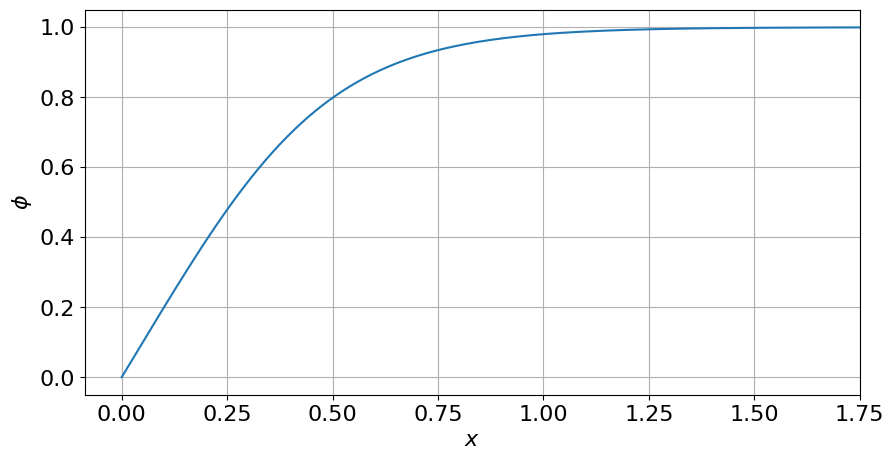
\includegraphics[width=0.89\textwidth]{pictures/result_volumes.png}
    \vspace{-0.3cm}
    \caption{Решение $\phi$ в плоском случае при $\alpha = 0, \; \beta = 0$.}
    \label{picture_result_volumes}
    \vspace{0.5cm}

    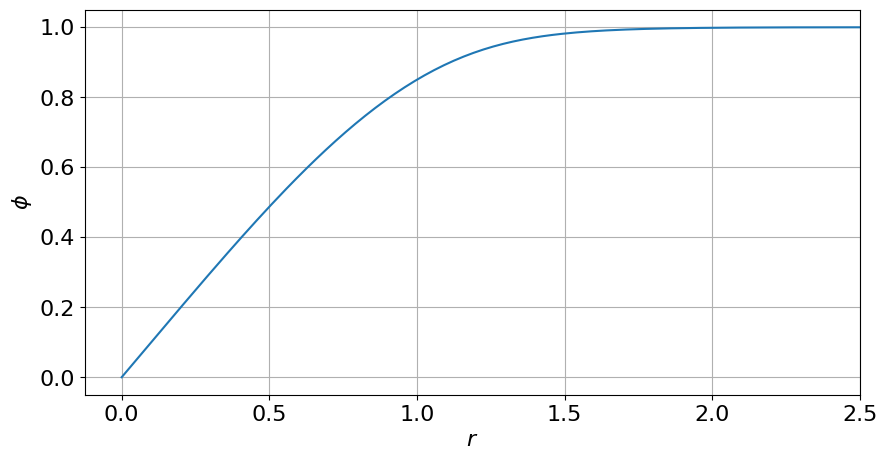
\includegraphics[width=0.89\textwidth]{pictures/result_volumes_p.png}
    \vspace{-0.3cm}
    \caption{Решение $\phi$ в плоском случае при $\alpha = 0, \; \beta = 1$.}
    \label{picture_result_volumes_p}
    \vspace{0.5cm}
    
    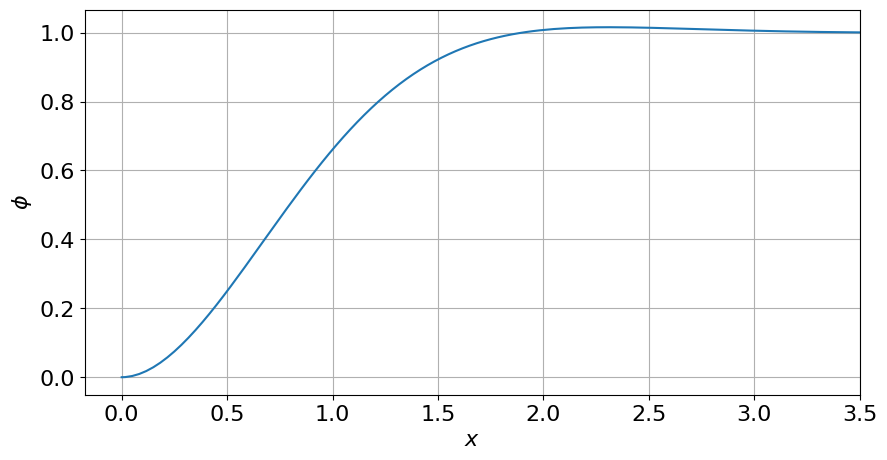
\includegraphics[width=0.89\textwidth]{pictures/result_volumes_bi.png}
    \vspace{-0.3cm}
    \caption{Решение $\phi$ в плоском случае при $\alpha = 1, \; \beta = 0$.}
    \label{picture_result_volumes_bi}
\end{figure}

\begin{figure}[!tp]
    \centering
    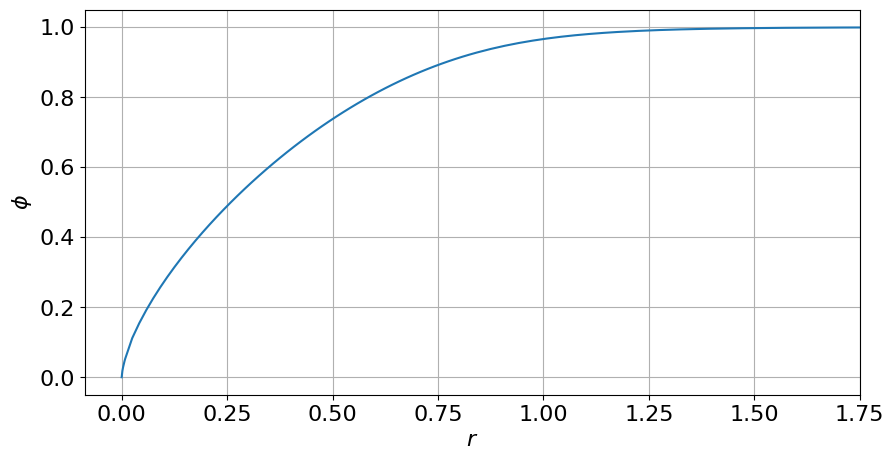
\includegraphics[width=0.89\textwidth]{pictures/result_volumes_cyl_p.png}
    \vspace{-0.3cm}
    \caption{Решение $\phi$ в цилиндрическом случае при $\alpha = 0, \; \beta = 1$.}
    \label{picture_result_volumes_cyl_p}
    \vspace{0.5cm}

    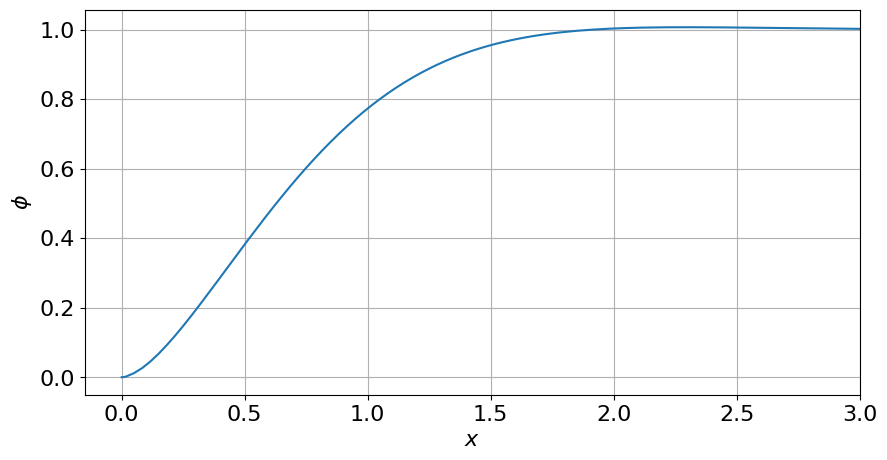
\includegraphics[width=0.89\textwidth]{pictures/result_volumes_cyl_bi.png}
    \vspace{-0.3cm}
    \caption{Решение $\phi$ в цилиндрическом случае при $\alpha = 1, \; \beta = 0$.}
    \label{picture_result_volumes_cyl_bi}
    \vspace{0.5cm}
    
    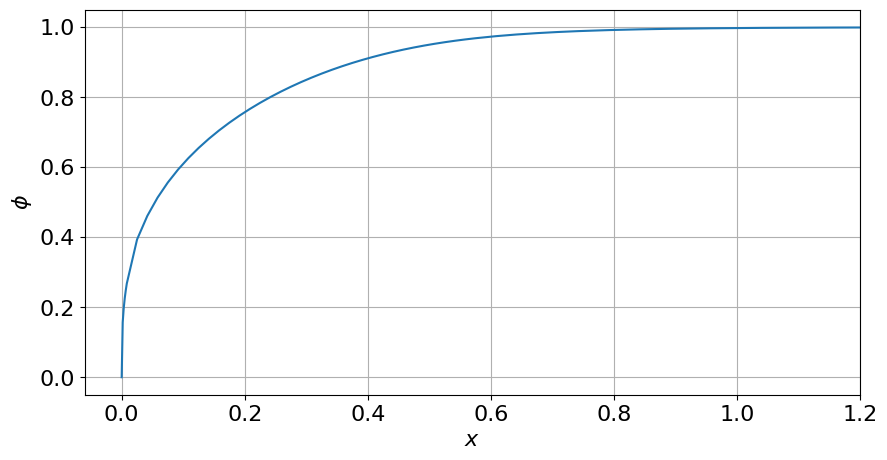
\includegraphics[width=0.89\textwidth]{pictures/result_volumes_sph_p.png}
    \vspace{-0.3cm}
    \caption{Решение $\phi$ в сферическом случае при $\alpha = 0, \; \beta = 1$.}
    \label{picture_result_volumes_sph_p}
\end{figure}

Отметим, что если в уравнения входит билапласиан ($\alpha \neq 0$), то функция $\phi$ может быть не монотонной и в некоторых точках превышать значение $1$ (см. рис. \ref{picture_result_volumes_bi}, \ref{picture_result_volumes_cyl_bi}). В работе \cite{zipunova_higher_codimension} это было отмечено и указано, что монотонность $\phi$ следует ожидать при достаточно малых $\alpha$.

Итак, эксперимент подтверждает, что, несмотря на некоторую громоздкость формулировок, предложенная модификация метода конечных объемов позволяет эффективно моделировать решение $\phi$, даже если на границе области оно имеет особенность.


\section{Заключение}

Моделирование развития канала электрического пробоя -- достаточно сложная задача. Использование модели типа диффузной границы, с одной стороны, несколько упрощает ее, позволяя не строить канал в виде геометрического объекта явно, однако с другой стороны, добавляет неясностей и вопросов, требующих ответа.

Настоящая работа -- попытка ответить на некоторые из этих вопросов. Большая часть исследования проделана численно; в численном анализе уже достигнуты определенные успехи и, кажется, виден простор для дальнейших изысканий.

Сложнее обстоит дело с теоретическим исследованием задачи. Существующая для подобного рода задач теория, во-первых, сложна, во-вторых, не позволяет провести их исчерпывающего анализа.

К основным результатам работы относятся следующие.
\begin{itemize}
    \item Проведен теоретический анализ модели.
    \item Построена разностная схема, дана содержательная оценка ее устойчивости; разработана  компьютерная программа, реализующая разностную схему; проведены вычислительные эксперименты, подтвердившие полученные результаты. 
    \item Рассмотрено обобщение исходной модели; на основе метода конечных объемов построена специальная разностная схема, учитывающая особенности решений на границе области моделирования; проведены соответствующие вычислительные эксперименты. На основании полученных результатов сделаны выводы и даны комментарии об эффекте, оказываемом рассмотренным обобщением модели.
\end{itemize}


\printbibliography

\end{document}
